% Compile with xelatex only.
% For bibliography, use biber
%
\documentclass[a5paper, 11pt, oneside, titlepage, numbers=endperiod]{scrbook}
%\documentclass[a4paper, 10pt,twoside,titlepage]{book} % swap for latex2rtf

\def \documentversion {1.2$\beta$}

% A switch to change between document rendering options
 \usepackage{etoolbox}
 \newtoggle{webpaper}
\toggletrue{webpaper}
%\togglefalse{webpaper}

\usepackage[top=1.5cm, bottom=2.2cm, left=1.84cm, right=1.5cm, footskip=1cm]{geometry}
\footskip=1.2cm

%\usepackage[utf8]{inputenc} % uncomment for latex2rtf 

\usepackage{ctable}  
\usepackage{caption}
\DeclareCaptionFormat{myformat}{\hfill#1#2\\ \bfseries#3}
\captionsetup[table]{justification=centering, singlelinecheck=off, format=myformat, labelformat = simple} % Ugly hack to remove prefix "table"

\usepackage{tikz}
\usetikzlibrary{shapes, calc, arrows, fit, positioning, decorations, patterns, decorations.pathreplacing, chains, snakes}

\usepackage{amsfonts}
\usepackage{amsmath}

\usepackage{csquotes}

\usepackage{polyglossia}

\usepackage{fontspec}
\defaultfontfeatures{Scale=MatchLowercase, Mapping=tex-text}
\newfontfamily\russianfont{CMU Serif}
\setromanfont{CMU Serif}
\setsansfont{CMU Sans Serif}
\setmonofont{CMU Typewriter Text}

\usepackage{xltxtra} % must be after fontspec
\setdefaultlanguage[spelling=modern]{russian}
\setotherlanguage{english}

\newcommand{\abbr}{\textit{англ.}\ }
\newcommand{\todo}{{\color{red}TODO}\ }
\usepackage{graphicx}
\graphicspath{{./images/}} % Путь к папке, содержащей рисунки

\tolerance=9999 % let the text underfull be ugly as hell, nobody cares.
\widowpenalty=9998 % try to avoid widow lines
\clubpenalty=9998 % try to avoid orphan lines
\emergencystretch=3em

\usepackage{hyperref}
\hypersetup{colorlinks=true, linkcolor=black, filecolor=black, citecolor=black, urlcolor=black , pdfauthor=Evgeny Yulyugin and Grigory Rechistov, pdftitle=Лабораторный практикум по программному моделированию}

\usepackage{footnpag}
\usepackage{indentfirst}
\usepackage{underscore}
\usepackage{longtable} 
\usepackage{url}

\usepackage{listings}
\lstset{basicstyle=\footnotesize\ttfamily, breaklines=true, keepspaces=true }

\iftoggle{webpaper}{
    % bibliography settings to put one after each chapter
    \usepackage[language=auto, bibencoding=inputenc, style=gost-numeric, backend=biber, maxnames=4, refsection=chapter]{biblatex}
} {
    % bibliography settings to put one global at the end
    \usepackage[language=auto, bibencoding=inputenc, style=gost-numeric, backend=biber, maxnames=4]{biblatex}
}

\usepackage[subfigure]{tocloft}
\renewcommand{\cftchapleader}{\cftdotfill{\cftdotsep}} % To set dots between chapter description and numbers
\setlength{\cftaftertoctitleskip}{20pt}

\usepackage{tabularx}

\usepackage{nameref}
\usepackage{amsthm}
\usepackage{enumitem} % continue enumeration 
\usepackage{subfigure}
\usepackage{mdwlist} % compact itemize lists environment
\usepackage{appendix}
\renewcommand{\appendixname}{Приложения}
\renewcommand{\appendixtocname}{Приложения}
\renewcommand{\appendixpagename}{Приложения}
\let\plainappendixpage\appendixpage
\makeatletter
\renewcommand{\appendixpage}{% Delete page number in appendixpage
  \begingroup
  \let\ps@plain\ps@empty
  \plainappendixpage
  \endgroup}
\makeatother

\renewcommand{\dictumwidth}{0.5\textwidth}
\newcommand{\dictumtext}{\normalfont\normalcolor\sffamily\tiny}
\setcounter{tocdepth}{2}

\usepackage{draftwatermark}
\SetWatermarkFontSize{35.83pt}
\SetWatermarkScale{3.0}

\addbibresource{./practicum.bib}
\renewcommand*{\multicitedelim}{\addcomma\space} % grouped cites separated by commas not semicolons

\addtokomafont{caption}{\small}
\renewcommand{\captionformat}{~} % do not put colon after figures numbers

\setkomafont{pagenumber}{\normalfont\rmfamily} % fix KOMA bug when footer/header inherits font settings from main text.

\usepackage{setspace}

\typeout{Copyright 2012, 2013, 2014 Grigory Rechistov and Evgeny Yulyugin.}
\begin{document}

\iftoggle{webpaper}{
    \pdfbookmark{Титульный лист}{title}

\thispagestyle{empty}
\vspace*{\stretch{1}}

\begin{center}
	\addfontfeature{LetterSpace=1.15}
	\huge\textsc{Лабораторный практикум по~программному моделированию}\par
	
	\bigskip
	
	\Large\textsc{Учебное пособие}
\end{center}

\vspace{\stretch{1}}

\newlength{\centeroffset}
\setlength{\centeroffset}{-0.5\oddsidemargin}
\addtolength{\centeroffset}{0.5\evensidemargin}

\noindent\hspace*{\centeroffset}\makebox[0pt][l]{
	\begin{minipage}{\textwidth}
		\flushright
		Версия~\documentversion \\
		\today\\[3cm]
	\end{minipage}
}
\pagebreak

\thispagestyle{empty}
\begin{small} 
Copyright \textcopyright~~2011, 2012, 2013, 2014 Grigory Rechistov, Yulyugin Evgeny.
\begin{center}
	
\includegraphics[width=0.2\textwidth]{cc-by-nc-sa.png}
\end{center}

Текст данного варианта произведения распространяется по лицензии Creative Commons At\-tri\-bu\-tion-Non\-Com\-mer\-cial-Share\-Alike (Атрибуция — Некоммерческое использование — На тех же условиях) 4.0 весь мир (в т.ч. Россия и др.). Чтобы ознакомиться с экземпляром этой лицензии, посетите \url{http://creativecommons.org/licenses/by-nc-sa/4.0/} или отправьте письмо на адрес Creative Commons: 171 Second Street, Suite 300, San Francisco, California, 94105, USA. 

Все зарегистрированные торговые марки, названия и логотипы, использованные в данных материалах, являются собственностью их владельцев. Представленная точка зрения отражает личное мнение авторов, не выступающих от лица какой-либо организации.
\end{small}

} {
    \pdfbookmark{Титульный лист}{title}

\thispagestyle{empty}

\begin{center}
\small
\textsc{Министерство образования и науки Российской Федерации \\
    Московский физико-технический институт \\
    (государственный университет) \\
}
\end{center}

\begin{center}
\textit{Кафедра радиоэлектроники и прикладной информатики}
\end{center}

\vfill

\begin{center}
    \begin{LARGE}
	\addfontfeature{LetterSpace=1.25}
    \textsc{Лабораторный практикум}\par
    \end{LARGE}
    \medskip
    \begin{Large}
	\addfontfeature{LetterSpace=1.25}
    \textsc{по программному моделированию}
    \end{Large}
\end{center}

\vfill

\begin{center}
\begin{large}
Составители: \\
\textit{\textbf{Е.А. Юлюгин, Г.C. Речистов, \\
    Н.Н. Щелкунов, Д.А. Гаврилов}}
\end{large}
\end{center}

\vfill

\begin{center}
    \textsc{Москва}\\
    \textsc{МФТИ}\\
    2013
\end{center}

    \thispagestyle{empty}
\begingroup
\small
\begin{flushleft}
УДК 004.42
\end{flushleft}

\begin{center}
\begin{normalsize}
\textsf{Р\,е\,ц\,е\,н\,з\,е\,н\,т}
\end{normalsize}

\medskip

Доктор технических наук, профессор кафедры информационных систем \\
управления и информационных технологий Московского государственного \\
университета приборостроения и информатики \textit{Т.~Ю.~Морозова}

\medskip

Кандидат технических наук, с.н.с., \\
начальник 4 отдела ОАО <<ИТМиВТ РАН>> \textit{Н.~Б.~Преображенский}

\end {center}

\textbf{Лабораторный практикум по программному моделированию}: учебно-методическое пособие / сост.: Е.~А.~Юлюгин, Г.~С.~Речистов, Н.~Н.~Щелкунов, Д.~А.~Гаврилов. --- М.: МФТИ, 2013. --- \pageref{page:lastpage}~с.\\

\medskip

Рассмотрены вопросы моделирования аппаратных средств однопроцессорных и многопроцессорных вычислительных систем. Основное внимание уделено технологиям построения программных симуляторов, в том числе на основе интерпретации, двоичной трансляции, аппаратной виртуализации, многопоточного исполнения и моделирования с использованием трасс. Учебное пособие подготовлено в «Лаборатории суперкомпьютерных технологий для биомедицины, фармакологии и малоразмерных структур» факультета радиотехники и кибернетики.

\medskip

Предназначено для студентов вузов, аспирантов и специалистов по средствам проектирования цифровых систем, разработке и исследованию проблемно-ориентированных архитектур ЭВМ и смежных направлений.

\vfill

\begin{center}
% The table in the bottom of the page.
\begin{tabular}{lp{0.6\textwidth}}
\hspace{4cm}                & \textcopyright~~Федеральное государственное автономное \\
                            & образовательное учреждение \\
                            & высшего профессионального образования \\
                            & «Московский физико-технический институт \\
                            & (государственный университет)», 2013
\end{tabular}

\end{center}

\endgroup

}

\begingroup
\setstretch{0.8}
\renewcommand\contentsname{Содержание}
\setcounter{tocdepth}{1}
\tableofcontents
\endgroup

\chapter*{Предисловие}\label{chap:contrib}

В настоящем практикуме описываются лабораторные и практические работы по курсу <<Основы программного моделирования ЭВМ>>, проводящиеся в Московском физико-техническом институте. Эта книга дополняет практическими аспектами программирования и использования технологий теоретические основы, изложенные в учебнике: 

Основы программного моделирования ЭВМ: Учебное пособие / Г. Речистов, Е. Юлюгин, А. Иванов, П. Шишпор, Н. Щелкунов, Д. Гаврилов. — 2-е изд., испр. и доп. — Издательство МФТИ, окт. 2013. — ISBN 978-5-7417-0444-8.

Авторы прикладывают усилия для того, чтобы поддерживать все учебные материалы в актуальном состоянии. Самую свежую версию данного документа вы можете получить на сайте \url{http://atakua.doesntexist.org/wordpress/simulation-course-russian/}.

Если вы обнаружили опечатку, стилистическую, фактическую ошибку, которые, более чем вероятно, встречаются в тексте, имеете замечания по содержанию или предложения по тому, как можно улучшить данный материал, то просим сообщить об этом по e-mail \url{grigory.rechistov@phystech.edu} --- нам очень важно ваше мнение!

Отметим, что текст данной работы постоянно обновляется, и поэтому в версиях, имеющих в своём номере пометку «бета» ($\beta$), могут присутствовать незаконченные места, которые обозначаются символом \todo.



% Don't show number of chapter in overview
\renewcommand{\thefigure}{\arabic{figure}}
\renewcommand{\thesection}{\arabic{section}}

\chapter*{Введение}\label{chap:overview}
\addcontentsline{toc}{chapter}{Введение} % This is a hack

\section{Компьютерная симуляция}

Использование компьютерного моделирования в процессе проектирования цифровых систем позволяет заметно сократить время, проходящее от момента предложения концепции новой системы до поступления на рынок первых образцов готовой продукции. Это происходит благодаря т. н. «сдвигу влево» (\textit{англ.} shift left) всей существующей методологии создания продукции, что позволяет выполнять ключевые процессы параллельно во времени, и значительноая часть из них может быть начата гораздо раньше, чем это было возможно ранее. Всё это эффективно сокращает длину цикла разработки нового продукта и увеличивает его конкурентноспособность (рис.~\ref{fig:shift-left}).

\begin{figure}[htb]
    \centering
    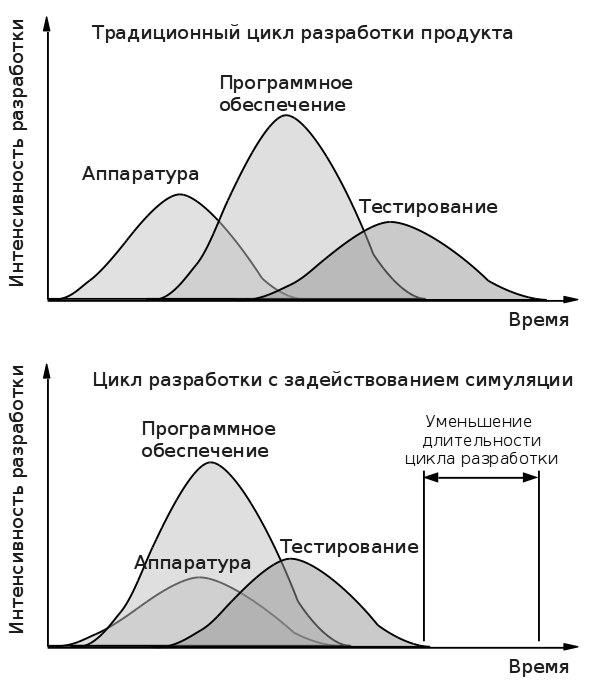
\includegraphics[width=0.7\textwidth]{./shift-left}
    \caption[Сдвиг влево]{Сдвиг влево --- возможность совместить моменты начала отдельных стадий проектирования новых цифровых систем, таким образом сокращая цикл разработки и уменьшая время вывода их на рынок}
    \label{fig:shift-left}
\end{figure}

Программное обеспечение для имитационного моделирования используется для тестирования функциональности, исследования производительности, оценки энергопотребления и иных свойств вычислительных систем на стадиях их раннего проектирования, когда реальные образцы соответствующей аппаратуры ещё недоступны. Кроме того, оно позволяет писать приложения для таких систем заранее и выпускать аппаратуру, готовую для использования конечным потребителем, не ожидая, пока все необходимые программы будут адаптированы.

Задача цикла лабораторных и практических работ, описанных в это книге, --- познакомить слушателей с новейшими достижениями в области компьютерной симуляции, связанными с эффективным созданием моделей, максимально точно представляющих аппаратные средства и при этом имеющих высокую скорость работы, получаемую благодаря эффективному задействованию имеющихся вычислительных ресурсов. Изучение проводится на программном продукте Wind River\textregistered\ Simics (в дальнейшем сокращённо называемого Simics), который в настоящее время является одним из самых современных инструментов разработки, тестирования и исследования цифровых компьютерных систем и используется как в промышленности, так и в научной среде. Несмотря на это, все рассматриваемые в книге вопросы основаны на концепциях, общих для многих других программных симуляторов, как коммерческих, так и исследовательских. В приложениях в конце книги дана информация о том, как подготовить компьютерный класс для выполнения лабораторных работ на Simics.

Для максимально эффективного усвоения материала данного пособия читателю рекомендуется иметь начальные знания по архитектуре ЭВМ. Желательно иметь понимание общих принципов работы операционных систем, а также знакомство с языками программирования высокого уровня и ассемблера. Базовой операционной системой для запуска приложений в практических работах служит GNU/Linux; для более чёткого понимания используемых в работах операций читатель должен быть знаком с работой интерпретатора командной строки Unix.

\section{Обозначения}
При первом использовании в тексте терминов, заимствованных из английского языка и не имеющих известных авторам общепринятых переводов на русский язык, в скобках после них будут указываться оригинальные выражения.

Всюду в тексте данной работы будут использованы следующие шрифтовые выделения и обозначения.

\begin{itemize*}
    \item Обычный текст используется для основного материала.
    \item \texttt{Моноширинный текст} вводится для исходных текстов программ на различных (псевдо) языках программирования и их ключевых слов,  имён регистров устройств, листингов машинного кода, результатов работы операторов командной строки.
    \item \textit{Курсивный текст} используется для выделения новых понятий.
    \item \textbf{Полужирный текст} используется для обозначения элементов графического интерфейса: имён окон, пунктов меню и т.п.
    \item Числа в шестнадцатеричной системе счисления имеют префикс \textbf{0x} (например, 0x12345abcd), в двоичной системе счисления --- суффикс \textbf{b} (например, 10010011b).
    \item Команды, которые необходимо вводить в строку приглашения запущенного Simics, имеют префикс \texttt{simics>}:
    \begin{lstlisting}
simics> list-objects
    \end{lstlisting}
	Ответный вывод команд, если он есть, приводится без каких-либо предваряющих префиксов. Если вывод очень длинен, то часть его заменяется многоточием.
    \item Команды, которые необходимо вводить в строку приглашения интерпретатора (в данной книге используется стандартный \texttt{/bin/sh}), имеют префикс \texttt{\$} для обычного пользователя или \texttt{\#} для команд, выполняемых суперпользователем root:
    \begin{lstlisting}
$ ./simics targets/x86-x58-ich10/viper.simics
# mount /dev/sdb /mnt/disk
    \end{lstlisting}

    \item При описании синтаксиса команд их обязательные аргументы команд указываются в угловых скобках, необязательные --- в квадратных:
    \begin{lstlisting}
$ command <mandatory argument> [optional argument]
    \end{lstlisting}
	Если команда принимает несколько однотипных аргументов подряд, спользуется многоточие \texttt{...} для второго и последующих параметров.
\end{itemize*}



\renewcommand{\thefigure}{\thechapter.\arabic{figure}}
\renewcommand{\thesection}{\thechapter.\arabic{section}}

\chapter{Первое знакомство с Simics}\label{chap:lab01}

\section{Цель занятия}

Ознакомиться с базовыми операциями, которые можно выполнять в рабочем окружении (\abbr workspace) симулятора Simics.

\begin{itemize*}
    \item Запуск симулятора. Элементы его интерфейса.
    \item Сценарии работы. Гостевые системы. 
    \item Процесс загрузки гостевой операционной системы внутри симулятора.
    \item Базовые операции: остановка модели, сохранение и восстановление симуляции с диска и на диск.
\end{itemize*}

\section{Запуск симулятора Simics. Элементы интерфейса}

% Wind River\textregistered\ Simics~\cite{getting-started} --- это быстрый, функционально точный полноплатформенный симулятор. Simics позволяет создать виртуальное окружение, в котором любая электронная система, начиная с одной платы и заканчивая целыми многопроцессорными и многоядерными системами, может быть определена, разработана и запущена.

Для запуска Simics на физическом \textit{хозяйском} компьютере архитектуры IA-32 должны быть установлены следующие программы.

\begin{itemize*}
\item Вариант операционной системы GNU/Linux. Simics может работать практически во всех современных дистрибутивах, включая Debian, Ubuntu, Fedora, OpenSUSE и др. Настоятельно рекомендуются 64-битные варианты ОС.
\item Графическая оболочка, любая из поддерживаемых выбранным дистрибутивом: KDE, Gnome, Fluxbox и др. Несмотря на то, что Simics может работать из чистой командной строки, далее всюду в тексте книги будет подразумеваться, что работа ведётся в графическом режиме.
\item Собственно копия Simics. По-умолчанию программа устанавливается в подкаталог \texttt{/opt/simics/simics-4.6}, который будет использоваться всюду в тексте.
\end{itemize*}

Подробнее об аппаратных требованиях к используемым компьютерам сказано в~\cite{installation}. Особенности централизованной установки Simics в компьютерном классе описаны в приложении~\ref{chap:installation-notes}.

\subsection{Создание Simics workspace}

Одна инсталляция Simics может быть использована совместно множеством пользователей; по этой причине её файлы должны оставаться неизменными. Рабочее окружение (\abbr <<workspace>>\footnote{Начиная с Simics версии 4.8 название workspace было сменено на project, однако мы будем использовать традиционную терминологию.}) --- это персональная <<копия>> общей установки, в которой Simics хранит ваши собственные настройки симуляционной среды, сценарии для конфигурации гостевых систем, двоичный и исходный код моделей и прочие данные. Каждый пользователь может иметь несколько независимых workspace, все они могут использоваться одновременно и независимо друг от друга и содержать различные окружения.

\subsubsection{Создание workspace}

Для создания нового workspace необходимо выполнить следующую последовательность действий.

\begin{enumerate*}
    \item Создайте директорию, в которой будет находиться новый workspace (рекомендуется использовать локации внутри домашней директории \texttt{\$HOME}) и перейдите в неё:

\begin{lstlisting}
$ mkdir <folder_name>
$ cd <folder_name>
\end{lstlisting}
    \item Вызовите программу workspace-setup из инсталляции Simics. Учтите, что путь к инсталляции и версия Simics может отличаться.
\begin{lstlisting}
$ /opt/simics/simics-4.6/simics-4.6.32/bin/workspace-setup
Workspace created successfully
\end{lstlisting}
\end{enumerate*}

Новый workspace создан! Текущая директория теперь содержит несколько файлов и поддиректорий:
\begin{lstlisting}
$ ls -1
bin
compiler.mk
config.mk
doc-cache
GNUmakefile
modules
simics
simics-gui
targets
\end{lstlisting}


\subsection{Запуск Simics}

После создания workspace вы можете начинать работу с Simics. Запустить симулятор вы можете с помощью команды:

\begin{lstlisting}
./simics
\end{lstlisting}

Должно открыться окно управления \textbf{Simics Control}\footnote{Последние версии Simics используют в качестве базового графического окружения среду Eclipse~\cite{eclipse}. Поддержка предыдущего, классического интерфейса была сохранена в полной мере. В этой книге мы всюду будем использовать только его.} (рис.~\ref{fig:simics-control}). Оно включает в себя иконки панели инструментов и меню, позволяющее контролировать состояния симулятора и текущей гостевой системы. Для выполнения данных лабораторных работ нам понадобится дополнительное окно с командной строкой \textbf{Simics Command Line} (рис.~\ref{fig:simics-command-line}). Выберите \textbf{Tools $\to$ Command Line Window} для того, чтобы открыть его.

\begin{figure}[ht]
    \centering
    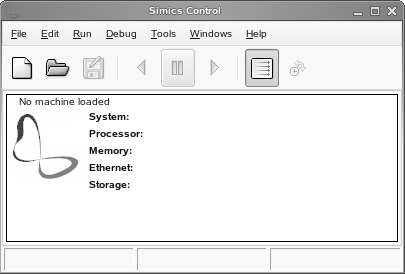
\includegraphics[width=0.6\textwidth]{./simics-control.png}
    \caption{Окно Simics Control}
    \label{fig:simics-control}
\end{figure}

\textbf{Simics Command Line} позволяет вам управлять симуляцией с помощью ввода текстовых команд. Во время своей работы Simics будет выводить в него диагностическую информацию: события симулятора и моделей, сообщения об ошибках и прочее. Всё, что можно сделать с помощью окна \textbf{Simics Control}, вы также можете сделать и с помощью командной строки. Большинство действий в дальнейшем будет производиться именно в ней.

\begin{figure}[ht]
    \centering
    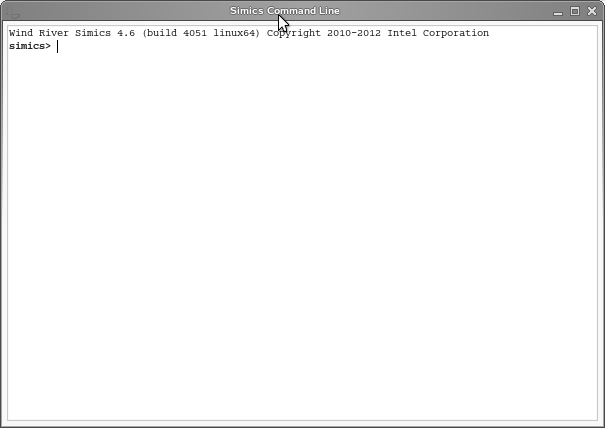
\includegraphics[width=0.6\textwidth]{./simics-command-line.png}
    \caption{Командная строка Simcs}
    \label{fig:simics-command-line}
\end{figure}

В данной главе в качестве моделируемой --- \textit{гостевой} --- используется вычислительная платформа, основанная на процессоре Intel\textsuperscript{\textregistered} Core\textsuperscript{\texttrademark} i7. GNU/Linux используется в качестве операционной системы. В качестве системной среды пользователя выступает пакет под названием BusyBox~\cite{BusyBox}, часто используемый во встраиваемых (\abbr embedded) системах.

Для загрузки конфигурации модели воспользуйтесь окном \textbf{Simics Command Line} и введите команду:

\begin{lstlisting}
simics> run-command-file targets/x86-x58-ich10/viper-firststeps.simics
\end{lstlisting}

То же самое можно было сделать с помощью окна \textbf{Simics Control}, выбрав \textbf{File $\to$ New session from script} и открыв файл \texttt{viper-firststeps.simics}, лежащий в директории \texttt{x86-x58-ich10}.

Спустя некоторое время окно \textbf{Simics Control} покажет суммарную информацию о симулируемой системе (рис.~\ref{fig:viper-control}): тип процессора, объём памяти, диска. Также должно открыться новое окно \textbf{Serial Console on viper.mb.sb.com[0]} (рис.~\ref{fig:viper-serial-console}).

\begin{figure}[ht]
    \centering
    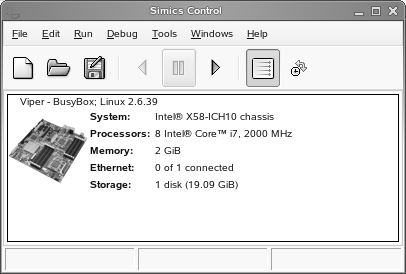
\includegraphics[width=0.6\textwidth]{./viper-control.png}
    \caption{Окно Simics Control после загрузки модели}
    \label{fig:viper-control}
\end{figure}

\begin{figure}[ht]
    \centering
    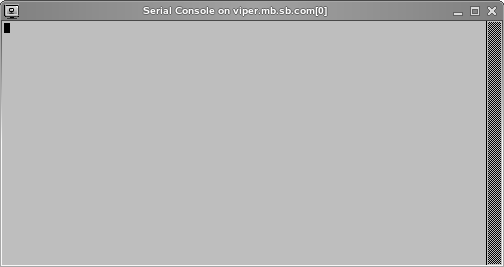
\includegraphics[width=0.6\textwidth]{./viper-serial-console.png}
    \caption[Окно Serial Console]{Окно \textbf{Serial Console on viper.mb.sb.com[0]}}
    \label{fig:viper-serial-console}
\end{figure}

Это новое окно является частью симуляции. Оно соединено с последовательным портом моделируемой материнской платы. Вывод сообщений гостевого ПО будет отображаться в нём. Кроме того, через него вы сможете взаимодействовать с моделируемым программным обеспечением, тогда как \textbf{Simics Command Line} используется для управления симуляцией.

\subsection{Запуск моделирования}

Теперь Simics ожидает ваших команд, вводимых через панель инструментов или через командную строку. Вы можете запустить симуляцию с помощью нажатия кнопки $\triangleright$ \textbf{Run Forward} на панели инструментов или ввода команды \texttt{continue} в командной строке.

Рассмотрим следующий пример:

\begin{lstlisting}
simics> continue
\end{lstlisting}

Для паузы симуляции в любой момент наберите команду \texttt{stop}.

\begin{lstlisting}
running> stop
[viper.mb.cpu0.core[0][0]] cs:0xffffffff8100944d p:0x00100944d  MWait state
simics>
\end{lstlisting}

После запуска симуляции виртуальное время (указываемое в нижней части \textbf{Simics Control}) начинает увеличиваться, инструкции гостевого процессора исполняются, и сообщения от программного обеспечения выводятся в окно консоли. Если вы позволите модели поработать некоторое время, то увидите сообщения от загрузки гостевой ОС в окне \textbf{Serial Console on viper.mb.sb.com[0]} (рис.~\ref{fig:booted-linux}). Симуляция может быть остановлена с помощью команды \texttt{stop} или нажатия \textbf{Stop} на панели инструментов.

\begin{figure}
	\centering
	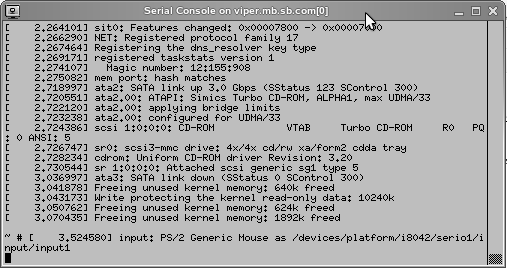
\includegraphics[width=0.6\textwidth]{./booted-linux.png}
	\caption{Загруженная операционная система Linux}
	\label{fig:booted-linux}
\end{figure}

После полной загрузки ОС в гостевой консоли будет выведено приглашение для логина пользователя:
\begin{lstlisting}
busybox login:
\end{lstlisting}

Введите в него \texttt{root}, нажмите \textbf{Enter}. Теперь гостевая операционная система загружена, и вы можете начать взаимодействовать с ней --- вводить инструкции в командной строке.

\paragraph{Получить листинг корневой директории.} Пример вывода команды \texttt{ls}:

\begin{lstlisting}
# ls /
bin      etc      host     linuxrc  root     sys
dev      home     init     proc     sbin     var
\end{lstlisting}

\paragraph{Увидеть информацию о моделируемом процессоре.} Пример содержимого псевдофайла \texttt{/proc/cpuinfo} гостевой системы:

\begin{lstlisting}
~ # cat /proc/cpuinfo                                                           
processor       : 0                                                             
vendor_id       : GenuineIntel                                                  
cpu family      : 6                                                             
model           : 26                                                            
model name      : Intel(R) Core(TM) i7 CPU     @ 2.00GHz               
stepping        : 8                                                             
cpu MHz         : 1999.991                                                      
cache size      : 8192 KB                                                       
fpu             : yes                                                           
fpu_exception   : yes                                                           
cpuid level     : 11                                                            
wp              : yes                                                           
flags           : fpu vme de pse tsc msr pae mce cx8 apic sep mtrr pge mca cmov 
pat pse36 clflush dts acpi mmx fxsr sse sse2 ss tm pbe syscall nx rdtscp lm cons
tant_tsc up arch_perfmon pebs bts rep_good nopl xtopology nonstop_tsc aperfmperf
 pni dtes64 monitor ds_cpl vmx est tm2 ssse3 cx16 xtpr pdcm sse4_1 sse4_2 popcnt
 lahf_lm ida dts tpr_shadow ept                                                 
bogomips        : 3999.98                                                       
clflush size    : 64                                                            
cache_alignment : 64                                                            
address sizes   : 36 bits physical, 48 bits virtual                             
power management:                                                               
\end{lstlisting}

Для того чтобы закончить работу симулятора, необходимо выполнить команду \texttt{quit}. Более подробно о командах Simics рассказывается в последующих главах, а также в приложении~\ref{chap:append01}.

\section{Сохранение и восстановление состояния симуляции}

\todo


% \section{Задания}

% \begin{enumerate*}
    % \item Загрузить модель Viper с операционной системой BusyBox~\cite{BusyBox}. Для этого необходимо из вашего workspace выполнить команду
% \begin{lstlisting}
% ./simics targets/x86-x58-ich10/viper-busybox.simics
% \end{lstlisting}
    % \item Открыть окно \textbf{Simics Command Line} и запустить симуляцию.
    % \item Сравнить содержимое файла \texttt{/proc/cpuinfo} симулируемой и реальной машины.
    % \item Найти способы определения факта нахождения внутри симулятора (имена устройств будут выдавать факт виртуализации).
% \end{enumerate*}

\section{Задания и контрольные вопросы к главе}

\begin{enumerate*}
\item Определите все отличия в параметрах аппаратных средств гостевой и хозяйской систем, используемых в данной работе. Какие средства могут быть использованы для обнаружения различий?
\item Сравните скорость течения виртуального времени, сообщаемого симуляцией, и настоящего времени. Чем, по-вашему, вызваны наблюдаемые различия?
\item Попытайтесь удалить \emph{все} файлы внутри симуляции. Каким образом это действие скажется на хозяйской системе? Перезапустите симуляцию. Что произошло с удалёнными файлами?
\end{enumerate*}

\iftoggle{webpaper}{
    \printbibliography[title={Список литературы к занятию}]
}{}


%%%%%%%%%%%%%%%%%%%%%%%%%%%%%%%%%%%%%%%% Legacy cluster.iscalare.mipt.ru notes %%%%%%%%%%%%%%%%%%%%%%%%%%%%%%%%%%%%%%%%%%%%%%%%%%%%%

% \subsection{Доступ на удалённую систему через SSH}\label{subsec:ssh}

% SSH (\abbr Secure SHell --- <<безопасная оболочка>>)~\cite{openssh} --- сетевой протокол прикладного уровня, позволяющий производить удаленное управление операционной системой и туннелирование TCP-соединений (например, для передачи файлов). SSH-клиенты и SSH-серверы доступны для большинства сетевых операционных систем.

% Ниже будут описаны способы использования SSH из-под операционных систем Linux и Windows.

% \subsubsection{Linux}

% Откройте терминал и наберите команду, заменив слово \texttt{user} на свой логин:

% \begin{lstlisting}
% $ ssh user@cluster.iscalare.mipt.ru
% \end{lstlisting}

% После этого система спросит у вас пароль. Введите его. Внимание! Вводимые символы не отображаются на экране. При удачном вводе пароля вы увидите сообщения приветствия командной строки (рис.~\ref{fig:ssh-login}).

% \subsubsection{Windows}

% Для того чтобы подключаться к удаленному серверу из системы Windows, необходимо воспользоваться SSH-клиентом, например, PuTTY~\cite{putty} (мы рекомендуем использовать именно его):

% \begin{enumerate*}
    % \item Запустите PuTTY.
    % \item В главном окне программы в поле \textbf{Host Name (or IP address)} введите строку \texttt{user@cluster.iscalare.mipt.ru}, заменив \texttt{user} на свой логин (рис.~\ref{fig:putty}).
    % \item Порт оставьте равным 22.
    % \item Сохраните сессию под некоторым именем, чтобы избежать необходимости повторного ввода в дальнейшем.
    % \item После открытия окна вам будет предложено ввести пароль. Введите его и нажмите \textbf{Enter}. Внимание: вводимые символы не отображаются на экране!
    % \item При удачном входе вы получите приглашение командной строки (рис.~\ref{fig:ssh-login}).
% \end{enumerate*}

% \begin{figure}[htb]
    % \centering
    % 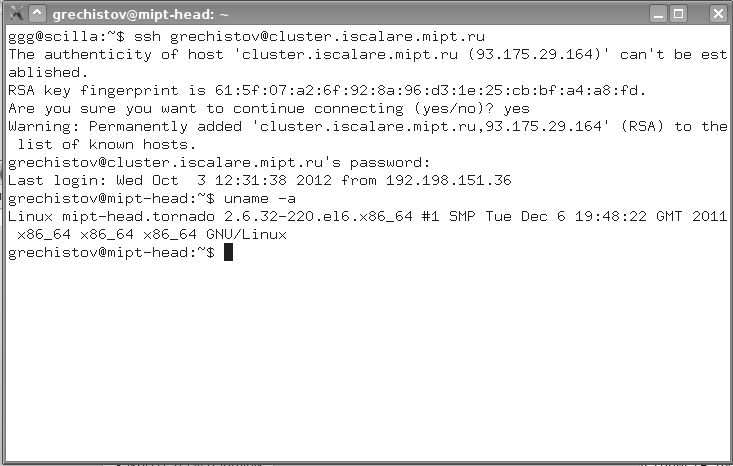
\includegraphics[width=0.6\textwidth]{./ssh-login}
    % \caption{Открытие сессии SSH}
    % \label{fig:ssh-login}
% \end{figure}

% \begin{figure}[htb]
    % \centering
    % 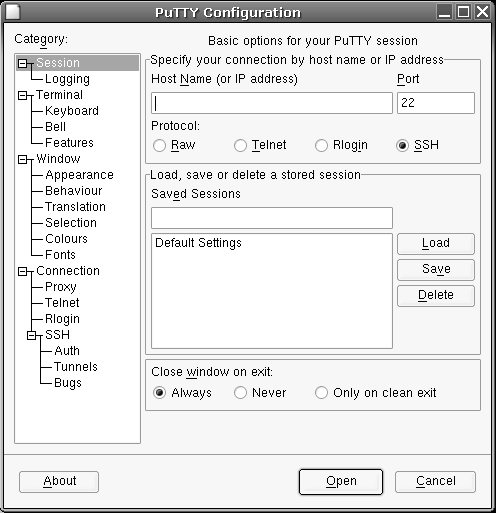
\includegraphics[width=0.6\textwidth]{./putty.png}
    % \caption{Окно PuTTY}
    % \label{fig:putty}
% \end{figure}

% \subsection{Создание VNC-сессии}

% VNC (\abbr Virtual Network Computing)~\cite{vnc} --- система удалённого доступа к рабочему столу компьютера, использующая протокол RFB (\abbr Remote Frame Buffer). VNC состоит из двух частей: клиента и сервера. Сервер — программа, предоставляющая доступ к экрану компьютера, на котором она запущена. Клиент (\abbr viewer) --- программа, получающая изображение экрана с сервера и взаимодействующая с ним по протоколу RFB. Управление осуществляется путём передачи нажатий клавиш на клавиатуре и движений мыши с одного компьютера на другой и ретрансляции содержимого экрана через компьютерную сеть. Система VNC платформонезависима: VNC-клиент, запущенный на одной операционной системе, может подключаться к VNC-серверу, работающему на любой другой ОС. Существуют реализации клиентской и серверной части практически для всех операционных систем, в том числе и для Java (включая мобильную платформу J2ME). К одному VNC-серверу одновременно могут подключаться множественные клиенты. Наиболее популярные способы использования VNC — удалённая техническая поддержка и доступ к рабочему компьютеру из дома.

% \subsubsection{Использование VNC для доступа к удаленному серверу}

% Для создани VNC-сессии необходимо выполнить следующую последовательность действий:

% \begin{enumerate*}
    % \item Зайдите на удалённый сервер, как описано в секции~\ref{subsec:ssh}.
    % \item Запустите команду для создания графического сервера с необходимым вам разрешением экрана:
% \begin{lstlisting}
% $ vncserver -geometry 1280x1024
% \end{lstlisting}
% Рекомендуется выбирать разрешение, равное или меньшее физического разрешения экрана вашей системы.
    % \item При необходимости (при первом запуске) задайте пароль (он не обязан совпадать с SSH-паролем). Пароль можно изменить впоследствии с помощью команды \texttt{vncpasswd}. Если вы забыли его, то удалить его можно, удалив файл \texttt{\$HOME/.vnc/passwd}.
    % \item Запомните номер сессии (число после двоеточия в выводе команды). Например, из вывода команды ниже видно, что только что созданный номер сессии равен 4.
% \begin{lstlisting}
% $ vncserver
% New 'mipt-head.tornado:4 (user)' desktop is mipt-head.tornado:4
% Starting applications specified in /home/user/.vnc/xstartup
% Log file is /home/user/.vnc/mipt-head.tornado:4.log
% \end{lstlisting}
% \textbf{Примечание.} Допускается иметь более одной VNC-сессии, при этом каждая будет иметь свой идентификатор (номер порта после двоеточия). Однако имейте в виду, что каждая из них потребляет небольшое количество общих системных ресурсов.
% Файл журнала соответствующей сессии, например \texttt{mipt-head.tornado:4.log}, полезен при анализе проблем при запуске, например, когда открываемый впоследствии графический экран пустой или VNC-сессия вообще не запустилась.
% \end{enumerate*}

% \subsubsection{Замечание о необходимости тунеллирования VNC}

% В настоящее время на \texttt{cluster.iscalare.mipt.ru} закрыты все внешние порты, кроме SSH (22). Поэтому для VNC-соединения, использующего порты в диапазоне 5901--5999, необходимо создавать т.н. \textbf{SSH-туннель}. Теоретически для локального конца туннеля можно выбирать любой порт (из непривилегированного диапазона 1001--65535), однако для избежания путаницы рекомендуется выбирать его равным номеру удалённого конца; в последующих примерах мы придерживаемся этого правила.

% \subsubsection{Отключение VNC-сессии}

% Обычно закрывать сессию VNC не требуется --- достаточно отключиться от неё. Затем можно возобновить работу, используя VNC-клиент. При необходимости уничтожение десктопа и всех запущенных приложений может быть выполнено командой

% \begin{lstlisting}
% $ vncserver -kill :4
% \end{lstlisting}

% Если необходимо уничтожить все свои VNC-сессии, используйте команду

% \begin{lstlisting}
% $ killall Xvnc
% \end{lstlisting}

% \subsubsection{Linux}

% Для начала нам необходимо установить VNC-клиент на наш рабочий компьютер (если он еще не установлен). Для установки клиента на персональную ЭВМ необходимо воспользоваться пакетным менеджером. Пример для Ubuntu/Debian:

% \begin{lstlisting}
% $ sudo apt-get install xtightvncviewer
% \end{lstlisting}

% Кроме того, допускается использовать любой клиент, поддерживающий протокол VNC: RealVNC, TighVNC, Remmina, Vinagre, Krdp\dots

% Затем используйте следующие опции \textbf{ssh} для создания туннеля (в примере ниже  --- для порта 5904, имени пользователя \texttt{user})

% \begin{lstlisting}
% $ ssh -L 5904:127.0.0.1:5904  -l user cluster.iscalare.mipt.ru
% \end{lstlisting}

% Если вы используете TightVNC, то для запуска VNC-сессии вам необходимо воспользоваться командой, указав после двоеточия номер вашей VNC-сессии (в данном примере номер VNC-сессии равен 4).

% \begin{lstlisting}
% $ vncviewer localhost:4
% \end{lstlisting}

% После этого система спросит у вас пароль. Введите его. Внимание! Вводимые символы не отображаются на экране. При удачном вводе пароля откроется окно VNC-сессии, готовое к работе. 

% \subsubsection{Windows}

% Для Windows мы рекомендуем использовать RealVNC. Инструкцию по установке и дополнительную информацию можно найти в~\cite{RealVNC}.

% Допускается использовать любой клиент, поддерживающий протокол VNC: RealVNC, TighVNC, UltraVNC\dots

% При открытии SSH из Putty дополнительно на складке Tunnels создаём проброс порта вашей VNC-сессии. В данном примере (рис.~\ref{fig:ssh-tunnel}) это экран VNC :4, что соответствует TCP-порту 5904.

% \begin{figure}[htb]
    % \centering
    % 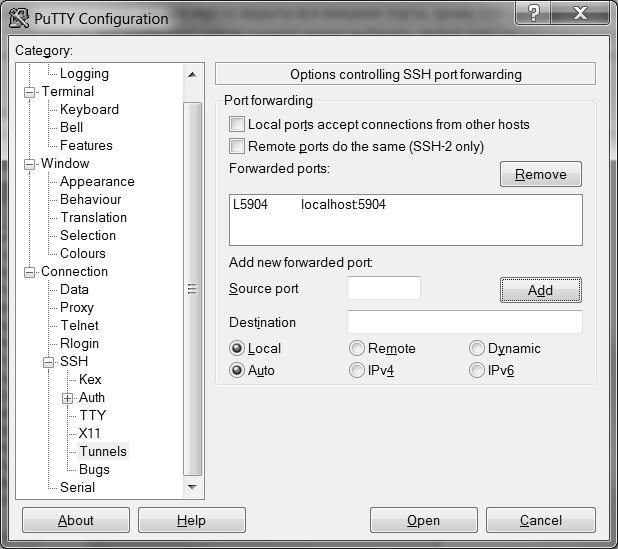
\includegraphics[width=0.6\textwidth]{./ssh-tunnel.png}
    % \caption{Создание ssh туннеля с помощью PuTTY}
    % \label{fig:ssh-tunnel}
% \end{figure}

% Для подключения к удаленному рабочему столу необходимо воспользоваться VNC-клиентом (в нашем примере это RealVNC). Выполните следующую последовательность действий:

% \begin{enumerate*}
    % \item Откройте VNC viewer.
    % \item В поле VNC Server укажите \textbf{localhost:4} (рис.~\ref{fig:realvnc}), заменив число 4 после двоеточия на номер вашей VNC-сессии.

% \begin{figure}[htb]
    % \centering
    % 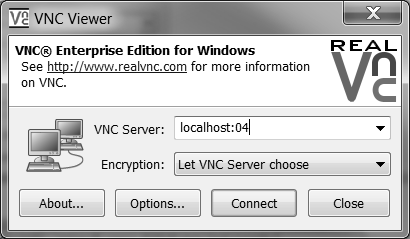
\includegraphics[width=0.5\textwidth]{./realvnc.png}
    % \caption{Окно RealVNC}
    % \label{fig:realvnc}
% \end{figure}

    % \item Нажмите \textbf{Connect}.
    % \item Система запросит ваш пароль от VNC-сессии. Введите его.
    % \item При удачном вводе пароля откроется окно VNC-сессии готовое к работе.
% \end{enumerate*}

% \subsection{Базовые команды Linux}

% В этой секции перечислены команды Linux, которые понадобятся для выполнения данной лабораторной работы:

% \begin{itemize*}
    % \item Команда \textbf{man} предназначена для формирования и  вывода справочной информации о команде \texttt{<command>}:
% \begin{lstlisting}
% $ man <command>
% \end{lstlisting}

    % \item Команда \texttt{ls} выводит информацию о \texttt{<file>} (по умолчанию выводится информация о текущей директории).
% \begin{lstlisting}
% $ ls <file>
% \end{lstlisting}

    % \item Команда \texttt{cd} меняет текущую рабочую директорию на \texttt{<directory>}.
% \begin{lstlisting}
% $ cd <directory>
% \end{lstlisting}

    % \item Команда \texttt{mkdir} создает директорию \texttt{<directory>} в текущей, если она до этого не существовала.
% \begin{lstlisting}
% $ mkdir <directory>
% \end{lstlisting}

    % \item Команда \texttt{cat} направляет \texttt{<file>} на стандартный вывод. Чаще всего это означает распечатывание его содержимого на экране.
% \begin{lstlisting}
% $ cat <file>
% \end{lstlisting}

    % \item Команда \texttt{lspci} показывает список всех PCI-устройств.
    % \item Команда \texttt{mount [node] <folder>} монтирует файловую систему; вызванная без аргументов, она перечисляет уже смонтированные системы.
    % \item Команда \texttt{umount <folder>} предназначена для отмонтирования файловой системы.
% \end{itemize*}

% Больше информации о командах Linux вы можете найти в мануалах, воспользовавшись командой \textbf{man}, описанной выше.


\chapter{Концепции симуляции}\label{chap:lab02}

\section{Цель занятия}

В данной работе продолжается изучение принципов работы симулятора Simics. Центральная тема занятия --- определение способов представления сущностей реальных устройств и систем в программных моделях.

\subsection{Базовая единица симуляции} 

Аналогично тому, что физические системы строятся из узлов, программные платформы состоят из моделей отдельных узлов. При этом, как и в реальности, они образуют иерархическую структуру.

\subsection{Диагностические сообщения}

Одно из назначений симуляторов --- помогать в разработке аппаратуры и программ для неё. При этом разработчикам необходимо понимать, что происходит в системе в определённые моменты времени. Для этого всем моделям позволено создавать диагностические сообщения, которые могут выводится на консоль управления Simics, а также в файл. Поскольку излишне частые и подробные сообщения могут засорить журнал, Simics предоставляет несколько механизмов для их фильтрации.

\section{Ход работы}

Запустите симулятор с моделируемой системой внутри:

\begin{lstlisting}
$ ./simics -e '$cpu_class=core-i7-single' targets/x86-x58-ich10/viper-busybox.simics
\end{lstlisting}

\subsection{Иерархия устройств}

Корневой элемент созданной модели компьютера имеет имя, хранящееся в переменной \texttt{\$system}. В нашем случае это \texttt{viper} --- модель шасси, на котором <<крепятся>> все остальные устройства. Этот факт выражается в том, что иерархические имена подкомпонент образованы присоединением к имени надкомпоненты своего имени через символ точки. Так, материнская плата данной системы имеет имя \texttt{viper.mb}, процессор на ней --- \texttt{viper.mb.cpu0}, а первое ядро в этом процессоре --- \texttt{viper.mb.cpu0.core[0][0]}.

Для просмотра списка всех устройств используйте команду \texttt{list-objects -recursive}. Альтернативно можно использовать окно \textbf{Object Browser} (рис.~\ref{fig:object-browser}).

\begin{figure}[htb]
    \centering
    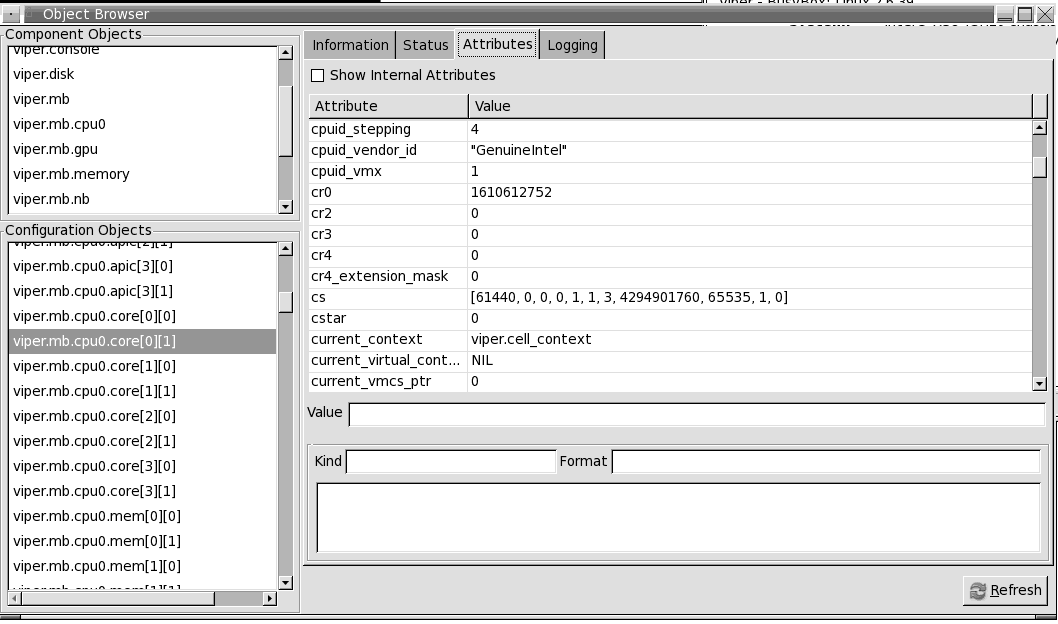
\includegraphics[width=0.8\textwidth]{/win-object-browser}
    \caption{Окно для просмотра объектов и их атбрибутов}
    \label{fig:object-browser}
\end{figure}


\subsection{Команды}

Каждый класс моделей может предоставлять несколько команд, которые позволяют инспектировать или изменять состояние объектов данного класса. Такие команды приписываются к иерархическому имени модели.

Самые часто реализуемые внутри классов команды --- это \texttt{status} и \texttt{info}.

Так же все устройства модели памяти имеют команды \texttt{get} и \texttt{set}, которые позволяют читать и записывать данные в симулируемую память. Например:

\begin{lstlisting}
simics> viper.mb.cpu0.mem[0][0].get address = 0xffff0000

simics> viper.mb.cpu0.mem[0][0].set address = 0xffff0000 value = 0xaabbccdd
\end{lstlisting}


\subsubsection{Глобальные команды}

Кроме команд, специфичных для устройств, существуют так называемые глобальные команды, эффект которых состоит или в доступе к состоянию всей симуляции в целом, или же к текущему <<устройству>> некоторого класса, что позволяет сэкономить время на наборе иерархических имён. Например, команда \texttt{ptime} выводит значения симулируемого времени для текущего процессора, тогда как \texttt{ptime -all} позволяет увидеть аналогичную информацию о всех процессорах в системе.

\begin{lstlisting}
simics> ptime
processor                 steps   cycles   time[s]
viper.mb.cpu0.core[0][0]      0        0         0
\end{lstlisting}


\subsection{Атрибуты}

Атрибуты являются аналогом полей классов в парадигме ООП. В симуляции основная их задача состоит в хранении архитектурного состояния моделей. Обратиться к ним можно по их имени, указываемому после имени объекта, с помощью оператора <<\texttt{->}>>:

Например, для просмотра регистров центрального процессора можно использовать соответствующие атрибуты:
\begin{lstlisting}
simics> viper.mb.cpu0.core[0][0]->rax
0
simics> viper.mb.cpu0.core[0][0]->rip
65520
simics> viper.mb.cpu0.core[0][0]->rdx
67233
simics> viper.mb.cpu0.core[0][0]->xmm
[[0, 0], [0, 0], [0, 0], [0, 0], [0, 0], [0, 0], [0, 0], [0, 0], [0, 0], [0, 0], [0, 0], [0, 0], [0, 0], [0, 0], [0, 0], [0, 0]]
\end{lstlisting}

Для изменения значения, хранимого в атрибуте, используется оператор присваивания <<\texttt{=}>>:
\begin{lstlisting}
simics> viper.mb.cpu0.core[0][0]->rax = 123
\end{lstlisting}

\subsubsection{Типы атрибутов}

По аналогии с переменными в языках программирования атрибуты имеют типы. При присвоении атрибуту нового значения предварительно производится проверка, что тип выражения с правой стороны соответсвует его заявленному типу.

Типы атрибутов специфицируются с помощью строки, символы которой определяют допустимые варианты входных значений.

\begin{enumerate*}
\item Скалярные. Имеют типы \texttt{i}, \texttt{s}, \texttt{b}.
\item Объекты. Их тип --- \texttt{o}.
\item Списки. Они могут быть как однородными \texttt{[iiii]}, так и содержать элементы разных типов \texttt{[oios]}. Кроме того, их длина может быть переменной: \texttt{[i*]}.
\item Пустой тип \texttt{n}.
\item Допустимо иметь атрибут, тип которого выбирается из нескольких ранее описанных: \texttt{i|s|o}.

\end{enumerate*}

Кроме того, некоторые атрибуты при регистрации могут быть помечены как псевдоатрибуты или атрибуты только для чтения. Почти всегда они не соответствуют архитектурному состоянию, а используются для удобства представления информации об устройстве или же могут быть выведены из содержимого других атрибутов.

\subsection{Интерфейсы}

Каждый интерфейс имеет уникальное имя и фиксированный набор методов, объединённых общей целью. Модель, желающая предоставлять некоторый интерфейс для других устройств, обязана реализовать один или несколько его методов и затем объявить его доступным. Стороннее устройство, имеющее ссылку на объект, может получить по нему заявленные интерфейсы и вызывать включённые в него методы. Таким образом, в Simics интерфейсы предоставляют объектно-ориентированную парадигму для взаимодействия отдельных моделей. 

Например, один из атрибутов процессора, настраиваемый на этапе инициализации модели, --- это \texttt{physical_memory}, его тип \texttt{o}, т.е. <<объект>>. Допустим, что \texttt{cpu->physical_memory = mem}. По указателю на объект \texttt{mem} процессор может извлечь из него реализацию интерфейса \texttt{memory-space}, который содержит методы \texttt{read}, \texttt{write}, \texttt{access} и др. для работы с пространствами памяти.

В данной работе мы не будем уделять много внимания  деталям работы с интерфейсами. Отметим лишь, что все команды любого устройства внутри себя написаны с использованием только его атрибутов и интерфейсов, т.к. не существует другого способа взаимодействий с ним. Однако устройства должны взаимодействовать друг с другом только через интерфейсы, но не атрибуты.

\subsection{Модули устройств}

С точки зрения организации хранения в Simics любая модель предоставляется ровно одним \textit{модулем} --- разделяемой библиотекой, загружаемой на этапе инициализации или позже. При этом модуль может предоставлять более одного класса моделей.

Для просмотра текущих загруженных модулей используйте команду:

\begin{lstlisting}
simics> list-modules -l
\end{lstlisting}

Для загрузки некоторого модуля вручную используется команда \texttt{load-module}.

Кроме того, некоторые найденные модули по той или иной причине могут быть отвергнуты при загрузке. Увидеть их список можно с помощью команды \texttt{list-failed-modules}.

% \subsection{Псевдоустройства}
% 
% Для унификации работы с различными сущностями в активной сессии Simics присутствуют также псевдоустройства, такие как \texttt{sim}, \texttt{prefs}, \texttt{sysmon} и др.

\subsection{Последовательность создания модели системы}

При создании симуляции она и все участвующие в ней объекты проходят две фазы, чётко отделённые друг от друга во времени, тогда как внутри каждой из них порядок инициализации компонент неопределён.

\begin{enumerate*}

\item \textit{Объявление} устройств и соединение их с помощью инициализации их атрибутов. На этом этапе ещё не произодится проверок на соответствие типов, наличие всех обязательных атрибутов. Устройства представлены так называемыми предобъектами (\abbr preobj).

\item \textit{Инстанциирование} устройств с помощью команды \texttt{instantiate-components}. На этом этапе производятся все проверки на корректность атрибутов, наличие необходимых интерфейсов. Если не найдено ошибок, то предобъекты преобразуются в полноценные объекты Simics, которые могут участввать в симуляции.

\end{enumerate*}

Отметим, что при необходимости добавить новые объекты в процессе симуляции описанные фазы могут быть повторены.

\section{Задания}

 В этой работе мы будем создавать небольшую симуляцию, состоящую из простой модели процессора класса \texttt{sample-risc} и модели оперативной памяти. Для этого необходимо будет создать и настроить индивидуальные объекты. Исходный скрипт находится в файле \texttt{script.py} (см. приложение~\ref{chap:app-broken-script}). Однако он содержит несколько ошибок, которые не позволяют это сделать сразу. Задание состоит в том, чтобы разобрать сообщения симулятора, внести модификации в исходный скрипт и запустить его.

Следующие замечания должны помочь в решении поставленной задачи.

\begin{itemize*}
    \item Данный скрипт написан на языке Python и поэтому требует специального флага при указании его имени в командной строке.
    \item Для выяснения списка опций используйте команду \texttt{simics -h}.
    \item Переменные в Simics объявляются с помощь оператора <<\texttt{=}>>. Имена переменных начинаются со знака доллар, например \texttt{\$system}.
    \item Перед выполнением второй фазы инициализации объектов все обязательные атрибуты предобъектов должны быть настроены.
    \item Обращайте внимание на вывод сообщения об ошибках --- часто они содержат имя файла и номер строки.
    \item Комментарии начинаются со знака <<диез>> \texttt{\#}.
\end{itemize*}

\iftoggle{webpaper}{
    \printbibliography[title={Список литературы к занятию}]
}{}

\chapter{Связь симуляции с внешним миром}\label{chap:lab03}

\section{Цель занятия}

Необходимость коммуникации --- доставка данных.

\begin{enumerate*}
    \item Образы дисков, форматы raw, craff, vmdk, iso.
    \item Паравиртуализация: hostfs, magic instructions.
    \item Сетевое взаимодействие: NAT, port forwarding, bridging.
\end{enumerate*}

\section{Диски}

Под дисками мы будем подразумевать устройства хранения данных на жёстких магнитных дисках (стандарты SATA, IDE, FireWire, SCSI), твердотельных накопителях (USB-флешки, SSD), а также оптические диски (CD, DVD, Blu-ray) и теряющие актуальность гибкие диски (\abbr floppy disks).

С моделированием дисковой подсистемы связано несколько специфичных вопросов.

\begin{itemize*}
\item Обеспечение высокой скорости симуляции. Объём передаваемых данных для ряда приложений может быть большим, как и связанное с этим замедление модели.
\item Обеспечение непосредственного хранения массивов данных. Ёмкость моделируемых дисков может достигать десятков терабайт.
\item Постоянство хранилища модели. В отличие от ОЗУ и регистров устройств, жёсткие диски не теряют данные при выключении или перезагрузке компьютера. Однако сохранение состояния между запусками симуляции нарушает принцип её воспроизводимости и повторяемости.
\end{itemize*}

\subsection{Форматы хранения}

Поскольку диск представляет собой устройство с произвольным доступом, естественная форма хранения его данных --- это файл в хозяйской системе. В простом случае он содержит собой просто копию байт-в-байт всего содержимого реального диска, т.н. «сырой» (\abbr raw) образ диска. Преимущество такого формата --- его простота и универсальность; практически все симуляторы поддерживают его. Основной недостаток --- нерациональное использование хозяйского дискового пространства. Например, симуляция установки ОС может занять 1 Гбайт места на образе диска в 100 Гбайт; результирующий образ диска будет занимать 100 Гбайт, при этом 99\% его будут потеряны для хозяйской системы впустую.

Многие симуляторы поддерживают более компактные способы хранения, в которых в файл записываются только изменённые секторы диска; заголовочная часть файла содержит список этих секторов и их местоположение. Как правило, каждая программа имеет свой формат и иногда поддерживает другие или позволяет конвертировать их друг в друга. Примеры: Qcow2~\cite{qcow2} (Qemu), VDI (Oracle Virtualbox), VMDK~\cite{vmdk} (VMware ESX), VHD (Microsoft VirtualPC), HDD (Parallels Desktop), CRAFF (Wind River Simics).

Некоторые форматы поддерживают прозрачное сжатие записанных данных.

Для образов оптических дисков, которые в большинстве  случаев являются носителями с данными только для чтения, используются сырые образы. Чаще всего они именуются ISO-образами по имени стандарта используемой на них файловой системы ISO 9660\footnote{Хотя это не единственный стандарт для оптических дисков; альтернативой является UDF (universal disk format), призванный обойти многие ограничения ISO 9660.}.

Из-за своего небольшого размера (меньше 3 Мбайт) образы гибких дисков хранятся в raw-формате.

\subsection{Сохранение состояния дисков}

Зачастую нежелательно модифицировать исходный файл образа диска: экспериментальное ПО/вирусы/ошибки пользователя внутри симулятора может сделать его неработоспособным, или же желательно впоследствии запускать симуляцию из первоначального состояния.

Для таких целей в большинстве симуляторов существует опция: все изменённые секторы сохранять не в оригинальном, а в дополнительном \textbf{разностном} файле (также называемом \textbf{дельтой}). Для моделируемого приложения указанная схема абсолютно прозрачна --- внутри симуляции изменения видны там, где и должны быть. Однако после выключения симуляции допустимо отбросить дельту и использовать оригинальный образ. В случае появления желания зафиксировать внесённые в результате последней симуляционной сессии правки --- следует воспользоваться утилитами слияния оригинального образа и дельты.

Развивая эту идею, можно вообразить себе схему с несколькими дельтами, полученными на разных этапах симуляции (и даже <<дельты к дельтам>>), одновременно наложенными на диск. Таким образом, можно иметь множество снимков состояний дискового хранилища, суммарно занимающие места меньше, чем занимали бы отдельные полные копии.

\section{Копирование файлов внутрь моделируемой системы}

Simics --- полноплатформенный симулятор, а это значит, что вся целевая система моделируется, включая диски, на которых установлено программное обеспечение. Часто может возникнуть необходимость транспортировки файлов из хозяйской системы в симулируемую и наоборот. Simics предоставляет способ прямого доступа к хозяйской операционной системе из моделируемой, называемой \textit{SimicsFS}.

\subsection{SimicsFS}

\textit{SimicsFS} --- это модуль ядра ОС, доступный в Linux и Solaris, для поддержки специальной файловой системы, делающий доступной файловую систему хозяина внутри гостевой системы. В рассматриваемой нами системе \textit{Viper} поддержка \textit{SimicsFS} уже установлена (описание процесса установки \textit{SimicsFS} можно найти в~\cite{hindsight}), поэтому для доступа к хозяйской файловой системе достаточно воспользоваться командой:

\begin{lstlisting}
# mount /host
[   25.060559] [simicsfs] mounted
\end{lstlisting}

После этого вы можете просматривать, скачивать и удалять файлы с хозяйской ЭВМ. Например, вы можете посмотреть содержимое корневой директории хозяйской операционной системы (Для Linux)

\begin{lstlisting}
# ls /host
bin     dev   ipathfs  lost+found  opt   sbin     share_debian  tmp
boot    etc   lib      media       proc  selinux  srv           usr
cgroup  home  lib64    mnt         root  share    sys           var
\end{lstlisting}

Вы можете сравнить вывод команды \texttt{ls /host} внутри моделируемой системы с выводом команды \texttt{ls /} внутри хозяйской системы и убедиться, что он совпадает.

Для того чтобы прекратить работу с \textit{SimicsFS}, достаточно просто отмонтировать хозяйскую файловую систему следующей командой:

\begin{lstlisting}
# umount /host
\end{lstlisting}

\subsection{Подключение симулятора к реальной сети}

Подключение симулятора к реальной сети открывает много новых возможностей. Например, позволяет упростить процесс загрузки файлов на симулируемую машину с помощью FTP (\abbr File Transfer Protocol); данная возможность может также использоваться для доступа к виртуальной машине удаленно с помощью Telnet.

\subsection{Типы соединений}

Simics предоставляет 4 способа подключения к реальной сети, которые описаны в~\cite{enug}. В данной секции описано, как они работают, их преимущества и недостатки.

\subsubsection{Перенаправление портов (\abbr Port forwarding)}

Перенаправление портов --- это самый простой тип соединений. Для установления соединения он не требует ни прав администратора, ни какой-либо другой конфигурации хозяйской машины.

Однако перенаправление портов ограничено только TCP- и UDP-трафиком. Другой трафик, например ping пакеты, которые использует ICMP-протокол, не пройдет через такое соединение. Нельзя использовать порты, которые уже используются на хозяйской машине, а также нельзя использовать порты меньше 1024 без прав администратора.

Каждый TCP- и UDP-порт требует отдельного правила перенаправления. По этой причине конфигурация приложений, которые используют множество портов или порты, определяемые произвольным образом (\abbr random ports), может оказаться довольно обременительной.

Перенаправление портов разрешает коммуникации между гостевой и хозяйской машинами, а также любыми узлами реальной сети.

\subsubsection{Соединение через сетевой мост (\abbr Ethernet bridging connection)}

С помощью соединения через сетевой мост у симулируемой машины появляеться возможность непосредственно подключаться к реальной сети. Данное соединение позволяет использовать трафик любого типа. Обычно симулируемый узел использует IP-адреса подсети, так как в данном случае не требуется менять конфигурацию хозяина. Тем не менее при использовании такого соединения хозяйская машина остается не доступной из гостевой.

Для использования соединения через сетевой мост на хозяйской машине необходимо иметь права на доступ к TAP.

\subsubsection{Соединение с хостом (\abbr Host connection)}

C помощью соединения с хостом хозяин подключается к моделируемой сети, позволяющей использование трафика любого типа между моделируемым и реальным узлами.

Соединение с хостом также поддерживает и перенаправление IP. Когда используется перенаправление IP, хозяйская операционная система маршрутизирует IP-трафик между реальной и симулируемой сетью. Из вышесказанного следует, что маршрутизация должна быть настроена между симулируемой и реальной сетью для того, чтобы данный способ работал.

Для использования соединения через сетевой мост на хозяйской машине необходимо иметь права на доступ к TAP.

\begin{table}[htb]
    \caption{Cпособы соединения с реальной сетью}
    \label{tab:cmp-real-network-connection}
    \center
    \begin{tabularx}{\textwidth}{|X|c|c|c|c|}
    \hline
        &   П. Портов   &   Мост Т  &   Мост НТ &   Хост \\
    \hline
    Права администратора для конфигурации   & нет   & да    & да    & да \\
    Права администратора для запуска    & нет   & нет   & да    & нет \\
    Реальный IP & нет   & да    & да    & нет \\
    Поддержка UDP/TCP   & да    & да    & да    & да \\
    Ограничение UDP/TCP-портами & да    & нет   & нет   & нет \\
    Поддержка всего IPv4    & нет   & да    & да    & да \\
    Поддержка всего Ethernet    & нет   & нет   & да    & да \\
    Соединение с хозяином   & да    & нет   & нет   & да \\
    Конфигурация хозяина    & нет   & нет   & да    & нет \\
    \hline
    \end{tabularx}

\begin{description*}
    \item[П. Портов:] перенаправление портов
    \item[Мост Т:] создание сетевого моста с трансляцией MAC-адресов
    \item[Мост НТ:] создание сетевого моста без трансляции MAC-адресов
    \item[Хост:] соединение с хостом
\end{description*}

\end{table}

Таблица~\ref{tab:cmp-real-network-connection} резюмирует преимущества и недостатки каждого типа соединений. Для простых TCP-сервисов, таких как FTP, HTTP или Telnet, лучше всего подходит перенаправление портов. В нашем случае этого достаточно, поэтому другие способы соединения с реальной сетью мы подробно рассматривать не будем.

Для каждого типа соединений с реальной сетью существет команда, которая принимает объект типа Ethernet link.

\section{Ход работы}

\subsection{SimicsFS}

\begin{enumerate*}

\item Загрузите Simics со стартовым скриптом \texttt{viper-busybox.simics} в конфигурации с процессором класса \texttt{core-i7-single}:
\begin{lstlisting}
$ ./simics -e '$cpu_class=core-i7-single' targets/x86-x58-ich10/viper-busybox.simics
\end{lstlisting}

\item Запустите симуляцию:
\begin{lstlisting}
simics> continue
running>
\end{lstlisting}

\item После того как гостевая система загрузится, авторизуйтесь и примонтируйте хозяйскую файловую систему:
\begin{lstlisting}
busybox login: root
[guest]# mount /host
\end{lstlisting}

\item Выведите содержимое корневой директории хозяйской операционной системы и сравните его с выводом содержимого папки /host внутри симулируемой машины:
\begin{lstlisting}
[host]$ ls /
[guest]# ls /host
\end{lstlisting}

\item Создайте файл в своей рабочей директории и убедитесь, что он также стал виден из симулируемой машины:
\begin{lstlisting}
[host]$ cd /share_debian/workspaces/students/ivanov
[host]$ touch test
[guest]# ls /host/share_debian/workspaces/students/ivanov
\end{lstlisting}

\item Удалите созданный файл из симулируемой машины и убедитесь, что в реальной системе он тоже был удален:
\begin{lstlisting}
[guest]# rm test
[host]$ ls /share_debian/workspaces/students/ivanov
\end{lstlisting}

\item Попробуйте из моделируемой системы удалить какой-либо системный файл хозяйской ОС, например, /bin/sh:
\begin{lstlisting}
[host]$ rm /bin/sh
rm: cannot remove `/bin/sh': Permission denied
[guest]# rm /host/bin/sh
rm: cannot remove `/host/bin/sh': Permission denied
\end{lstlisting}

Видно, что даже наличие прав администратора внутри симулируемого узла не позволяет нам удалять файлы, недоступные для записи пользователю, который запустил симуляцию.

\end{enumerate*}

\subsection{Подключение к реальной сети}

\begin{enumerate*}

\item Прежде чем подключать симулируемую систему к реальной сети, нам необходимо убедиться, что у хозяйской машины есть подключение к Интернету. В противном случае симулируемая система также не сможет подключиться к сети. Проверим, что соединение с Интернетом есть у реальной системы. Протестируем Telnet соединение с веб-сервером, например google.com, на 80 порту, с помощью ввода команды \texttt{GET /}. Эта команда должна вернуть HTML-содержимое стартовой странцицы сервера
\begin{lstlisting}
$ telnet www.google.com 80
Trying 74.125.232.243...
Connected to www.google.com.
Escape character is '^]'.
GET /
HTTP/1.0 302 Found
Location: http://www.google.ru/
Cache-Control: private
Content-Type: text/html; charset=UTF-8
Set-Cookie: PREF=ID=8ebf0b0d9fda87c2:FF=0:TM=1358767271:LM=1358767271:S=i7ZpIQ-KLg2H1VXZ;
expires=Wed, 21-Jan-2015 11:21:11 GMT;
path=/; domain=.google.com
Set-Cookie: NID=67=ogXTGYQQ5wlyfWupN8EmmGRdfL_7FQ5CNhU3yf2lArXX-04...
expires=Tue, 23-Jul-2013 11:21:11 GMT;
path=/; domain=.google.com; HttpOnly
P3P: CP="This is not a P3P policy! See http://www.google.com/support/accounts/bin/answer.py?hl=en&answer=151657 for more info."
Date: Mon, 21 Jan 2013 11:21:11 GMT
Server: gws
Content-Length: 218
X-XSS-Protection: 1; mode=block
X-Frame-Options: SAMEORIGIN

<HTML><HEAD><meta http-equiv="content-type" content="text/html;charset=utf-8">
<TITLE>302 Moved</TITLE></HEAD><BODY>
<H1>302 Moved</H1>
The document has moved
<A HREF="http://www.google.ru/">here</A>.
</BODY></HTML>
Connection closed by foreign host.
\end{lstlisting}

\item Загрузите Simics со стартовым скриптом \texttt{practicum.simics}~ref{chap:target-script}:
\begin{lstlisting}
$ ./simics targets/practicum.simics
\end{lstlisting}

\item На холостом ходу наша симулируемая машина может бежать быстрее реального времени, поэтому время ожидания соединения может пройти быстрее, чем требуется. Для того чтобы избежать этого, необходимо включить режим реального времени.
\begin{lstlisting}
simics> enable-real-time-mode
simics>
\end{lstlisting}

\item Подкулючите моделируемую систему к реальной сети с помощью команды connect-real-network
\begin{lstlisting}
simics> connect-real-network 192.168.1.100
No ethernet link found, created default_eth_switch0.
Connected practicum.mb.sb.eth_slot to default_eth_switch0
Created instantiated 'std-service-node' component 'default_service_node0'
Connecting 'default_service_node0' to 'default_eth_switch0' as 192.168.1.1
NAPT enabled with gateway 192.168.1.1/24 on link default_eth_switch0.link.
NAPT enabled with gateway fe80::2220:20ff:fe20:2000/64 on link default_eth_switch0.link.
Host TCP port 4021 -> 192.168.1.100:21
Host TCP port 4022 -> 192.168.1.100:22
Host TCP port 4023 -> 192.168.1.100:23
Host TCP port 4080 -> 192.168.1.100:80
Real DNS enabled at 192.168.1.1/24 on link default_eth_switch0.link.
Real DNS enabled at fe80::2220:20ff:fe20:2000/64 on link default_eth_switch0.link.
simics>
\end{lstlisting}

\item Необходимо включить DHCP pool. Переменная \texttt{service_node} должна создаться после выполнения команды \texttt{connect-real-network}:
\begin{lstlisting}
simics> default_service_node0.dhcp-add-pool pool-size = 50 ip = 192.168.1.150
simics>
\end{lstlisting}

\item Запустите симуляцию:
\begin{lstlisting}
simics> continue
running>
\end{lstlisting}

\item После загрузки симулируемого узла для доступа в Интернет необходимо настроить DHCP.
\begin{lstlisting}
user@master0:~$ sudo dhclient -v eth1                                           
Internet Systems Consortium DHCP Client 4.1.1-P1
Copyright 2004-2010 Internet Systems Consortium.
All rights reserved.
For info, please visit https://www.isc.org/software/dhcp/

[  121.257375] ADDRCONF(NETDEV_UP): eth1: link is not ready
[  121.261351] e1000e: eth1 NIC Link is Up 10 Mbps Full Duplex, Flow Control: No
ne
[  121.261764] 0000:00:19.0: eth1: 10/100 speed: disabling TSO
[  121.262438] ADDRCONF(NETDEV_CHANGE): eth1: link becomes ready
Listening on LPF/eth1/00:19:a0:e1:1c:9f
Sending on   LPF/eth1/00:19:a0:e1:1c:9f
Sending on   Socket/fallback
DHCPDISCOVER on eth1 to 255.255.255.255 port 67 interval 8
DHCPOFFER from 192.168.1.1
DHCPREQUEST on eth1 to 255.255.255.255 port 67
DHCPACK from 192.168.1.1
bound to 192.168.1.150 -- renewal in 1517 seconds.
user@master0:~$ 
\end{lstlisting}

\item
\begin{lstlisting}
user@master0:~$ telnet gnu.org 80
Trying 208.118.235.148...
Connected to gnu.org.
Escape character is '^]'.
GET /
<!DOCTYPE HTML PUBLIC "-//IETF//DTD HTML 2.0//EN">
<html><head>
<title>302 Found</title>
</head><body>
<h1>Found</h1>
<p>The document has moved <a href="http://savannah.nongnu.org/?">here</a>.</p>
<hr>
<address>Apache/2.2.14 Server at www.nongnu.org Port 80</address>
</body></html>
Connection closed by foreign host.
\end{lstlisting}

\item Также с помощью Telnet вы можете посмотреть ASCII-версию <<Звездных войн>>
\begin{lstlisting}
user@master0:~$ telnet towel.blinkenlights.nl
\end{lstlisting}

\end{enumerate*}

\iftoggle{webpaper}{
    \printbibliography[title={Список литературы к занятию}]
}{}

\chapter{Использование симуляции для отладки приложений}\label{chap:lab04}

В ходе данной лабораторной работы слушатели ознакомятся со способами изучения состояния симулируемой системы, отладки приложений, в том числе с символьной информацией, запущенных под управлением гостевой ОС.

Хотя для отладки приложений непосредственно на хозяйской системе существует достаточно широкий набор инструментов, например GDB~\cite{gdb}, WinDbg~\cite{windbg} и KВ, в ряде сценариев, таких как отладка системного кода BIOS или ОС, симуляция обеспечивает определённые удобства и преимущества, например, отсутствие необходимости использовать отдельную физическую машину для запуска отладчика. На ранних стадиях загрузки системы, когда никакой отладчик ещё не может быть подключен, моделирование является единственным решением.

Подробная информация о поддерживаемых методах отладки в Simics содержится в~\cite{analyzer, hindsight}.

\section{Цель занятия}

\begin{itemize*}
    \item Научиться подготавливать модель к символьной отладке приложений.
    \item Изучить команды инспектирования состояния гостевой системы.
\end{itemize*}

\section{Ход работы}

В приведённом ниже эксперименте мы будет изучать поведение гостевого приложения средствами инспектирования состояния и символической отладки, присутствующими в Simics. В нашем примере имя этого приложения --- \texttt{debug_example}.

\subsection{Подготовка исследуемой программы}

Исходный код программы \texttt{debug_example.c}, содержащей ошибку, находится в приложении~\ref{chap:debug-example}. Скомпилируйте \texttt{debug_example.c} для архитектуры x86, используя флаг \texttt{-m32}, и с включением отладочной информации в исполняемый файл, флаг \texttt{-g}.

\begin{lstlisting}
gcc -m32 -g -static debug_example.c -o debug_example
\end{lstlisting} 

\subsection{Подготовка гостевой системы}

\begin{enumerate}

\item Загрузите Simics со стартовым скриптом \texttt{viper-busybox.simics} в конфигурации с процессором класса \texttt{core-i7-single}:

\begin{lstlisting}
$ ./simics -e '$cpu_class=core-i7-single' targets/x86-x58-ich10/viper-busybox.simics
\end{lstlisting}

\item Включите режим обратного исполнения. Затем запустите симуляцию:
\begin{lstlisting}
simics> enable-reverse-execution
simics> continue
\end{lstlisting}

\item После того как гостевая система загрузится, авторизуйтесь и примонтируйте хозяйскую файловую систему и скопируйте файл изучаемого приложения внутрь гостя
\begin{lstlisting}
busybox login: root
~ # mount /host
~ # cp /host/home/user/debug_example ./
~ # chmod +x debug_example
\end{lstlisting}

\item Проверьте настройки отладчика запуском симуляции и командой:
\begin{lstlisting}
simics> viper.software.list
\end{lstlisting}

Вывод в консоль должен содержать список запущенных процессов на гостевой системе.
\begin{lstlisting}
Process Binary PID TID
kthreadd 2
migration/0 3
ksoftirqd/0 4
watchdog/0 5
migration/1 6
ksoftirqd/1 7
watchdog/1 8
events/0 9
events/1 10
khelper 11
async/mgr 14
sync_supers 98
bdi-default 100
kblockd/0 102
kblockd/1 103
kseriod 113
rpciod/0 132
rpciod/1 133
khungtaskd 159
kswapd0 160
aio/0 208
aio/1 209
nfsiod 217
crypto/0 223
crypto/1 224
flush-1:0 967
kjournald 957
init 1 1
sh 974 974
httpd 973 973
telnetd 971 971
\end{lstlisting}

\item Для того чтобы сконфигурировать отладчик, создайте объект символьной таблицы.
\begin{lstlisting}
simics> new-symtable debug_example
Created symbol table 'debug_example'
debug_example set for context viper.cell_context
\end{lstlisting}

\item Затем загрузите символьную информацию из исполняемого файла в созданный объект.
\begin{lstlisting}
simics> viper.software.track node = debug symtable = debug_example
Context debug0 will start tracking debug when it starts
simics> debug_example.load-symbols debug_example
\end{lstlisting}

\end{enumerate}

\subsection{Инспектирование состояния гостевой системы}

\subsubsection{Окно просмотра регистров}

Основное состояние центрального процессора хранится в его регистрах. Для просмотра регистров в Simics используется окно \textbf{CPU registers}, вызываемое через меню главного окна или через команду консоли \texttt{win-cpu-registers}. На рис.~\ref{fig:win-cpu-register-integer} и~\ref{fig:win-cpu-registers-system} показаны примеры содержимого двух вкладок этого окна. Также регистры можно просмотреть с помощью команды \texttt{pregs}:

\begin{lstlisting}
simics> pregs -all

64-bit mode
rax = 0x00007fff387d56a0             r8  = 0x000000000000000b
rcx = 0x0000000000000004             r9  = 0x000000000000000f
rdx = 0x00007fff387d5758             r10 = 0x000000000000000b
rbx = 0x0000000000400e30             r11 = 0x0000000000000008
rsp = 0x00007fff387d5660             r12 = 0x0000000000000000
rbp = 0x00007fff387d5670             r13 = 0x0000000000000000
rsi = 0x00007fff387d5748             r14 = 0x0000000000000000
rdi = 0x0000000000000001             r15 = 0x0000000000000000

rip = 0x00000000004004c3, linear = 0x00000000004004c3

eflags = 0 0 0 0 0 0 0 0 0 0 0 0 1 0 0 0 0 0 0 1 1 0 = 0x00000206
         I V V A V R - N I I O D I T S Z - A - P - C
         D I I C M F   T O O F F F F F F   F   F   F
           P F           P P                        
                         L L                        

es   = 0x0000, base = 0x00000000, limit = 0x0, attr = 0x0
cs   = 0x0033, base = 0x00000000, limit = 0xffffffff, attr = 0xa0fb
ss   = 0x002b, base = 0x00000000, limit = 0xffffffff, attr = 0xc0f3
ds   = 0x0000, base = 0x00000000, limit = 0x0, attr = 0x0
fs   = 0x0063, base = 0x02024860, limit = 0xffffffff, attr = 0xc0f3
gs   = 0x0000, base = 0x00000000, limit = 0x0, attr = 0x0
tr   = 0x0040, base = 0xffff88007fc0f900, limit = 0x2087, attr = 0x8b
ldtr   = 0x0000, base = 0x00000000, limit = 0xffff, attr = 0x82
idtr: base = 0xffffffff81b85000, limit = 00fff
gdtr: base = 0xffff88007fc04000, limit = 0007f

efer = 1 1 - 1 -- 1 = 0x00000d01
       N L   L    S
       X M   M    C
       E A   E    E

cr0 = 1 0 0 -- 1 - 1 -- 1 1 0 0 1 1 = 0x80050033
      P C N    A   W    N E T E M P
      G D W    M   P    E T S M P E

cr2 = 0x000000000040c930
cr3 = 0x000000007c01b000

cr4 = 0 - 1 1 0 1 1 1 1 0 0 0 0 = 0x000006f0
      V   O O P P M P P D T P V
      M   S S C G C A S E S V M
      X   X F E E E E E   D I E
      E   M X
          M S
          E R
          X
          C
          P
          T

dr0 = 0x0000000000000000 disabled
dr1 = 0x0000000000000000 disabled
dr2 = 0x0000000000000000 disabled
dr3 = 0x0000000000000000 disabled

dr6 = 0 0 0 -- 0 0 0 0 = 0xffff0ff0
      B B B    B B B B
      T S D    3 2 1 0

dr7 = 00000400

<Вывод опущен>
\end{lstlisting}

\begin{figure}[htb]
    \centering
    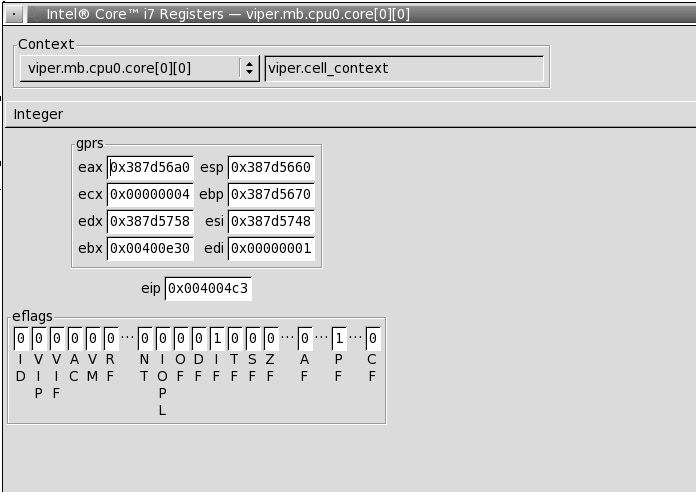
\includegraphics[width=0.6\textwidth]{./images/win-cpu-registers-integer.png}
    % win-cpu-registers-integer.png: 696x492 pixel, 96dpi, 18.41x13.02 cm, bb=0 0 522 369
    \caption{Окно просмотра регистров. Вкладка с регистрами общего назначения}
    \label{fig:win-cpu-register-integer}
\end{figure}

\begin{figure}[htb]
    \centering
    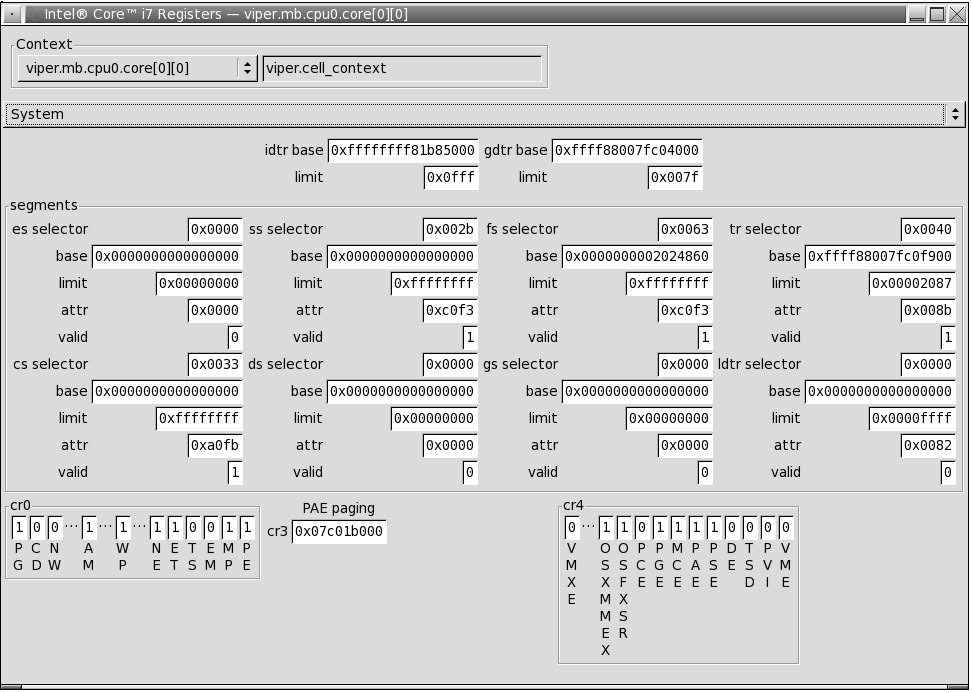
\includegraphics[width=0.8\textwidth]{./images/win-cpu-registers-system.png}
    % win-cpu-registers-system.png: 972x693 pixel, 96dpi, 25.71x18.33 cm, bb=0 0 729 520
    \caption{Окно просмотра регистров. Вкладка с системными регистрами}
    \label{fig:win-cpu-registers-system}
\end{figure}

\subsubsection{Память системы}

Для просмотра различных пространств памяти, присутствующих в моделируемой системе, используется окно \textbf{Memory Contents}, вызываемое также командой \texttt{win-memory} (рис.~\ref{fig:win-memory}).

\begin{figure}[htb]
    \centering
    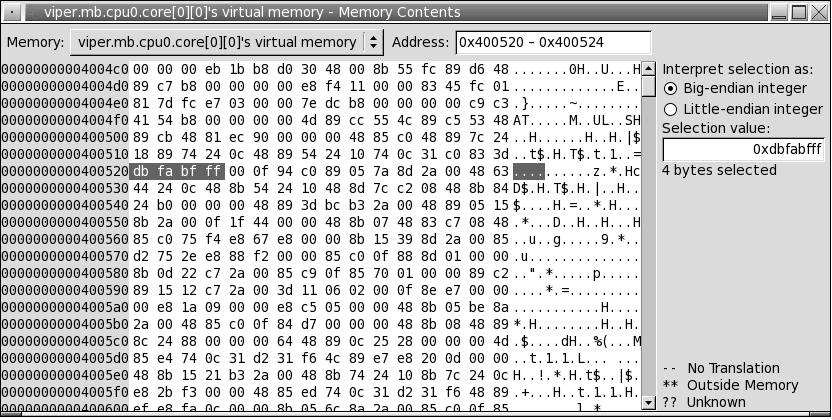
\includegraphics[width=0.8\textwidth]{./images/win-memory.png}
    % win-memory.png: 832x420 pixel, 96dpi, 22.01x11.11 cm, bb=0 0 624 315
    \caption{Окно просмотра содержимого памяти системы}
    \label{fig:win-memory}
\end{figure}

\subsection{Начало отладки}

Поставьте точку останова на функции \texttt{main()} и запустите симуляцию.
\begin{lstlisting}
simics> break (pos main) -x
Breakpoint 92 set on address 0x80485c6 in 'viper.cell_context' with access mode 'x'
simics> continue
\end{lstlisting}

В гостевой ОС запустите исполняемый файл \texttt{debug_example}. Симуляция должна остановиться с выводом в консоль:
\begin{lstlisting}
Breakpoint 922 on instruction fetch from 0x80485c6 in viper.cell_context.
[viper.mb.cpu0.core[0][1]] cs:0x00000000080485c6 p:0x07c17e5c6  lea ecx,4[esp]
Setting new inspection cpu: viper.mb.cpu0.core[0][1]
main (argc=, argv=) at /nfs/ims/home/mvchurik/working_folder/debug_example.c:53
53      (file /nfs/ims/home/mvchurik/working_folder/debug_example.c not found)
\end{lstlisting}

% Перейдите к окну отладки.
\begin{lstlisting}
simics> win-source-view
\end{lstlisting}
Убедитесь, что поле \textbf{Source File}  окна \textbf{Source Code} (рис.~\ref{fig:win-source-view}) заполнено. В противном случае загрузите в окно исходный файл кнопкой \textbf{Find}.

\begin{figure}[htb]
    \centering
    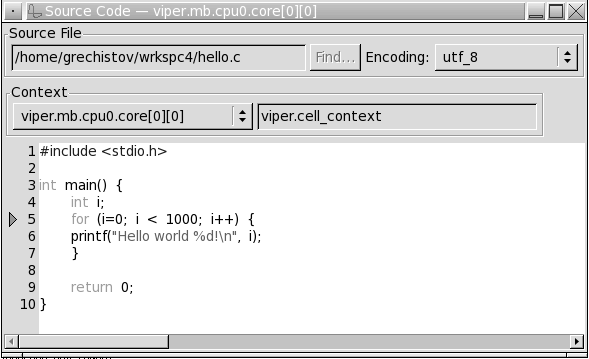
\includegraphics[width=0.6\textwidth]{./win-source-view.png}
    \caption{Окно просмотра исходного кода}
    \label{fig:win-source-view}
\end{figure}

\subsection{Окна с информацией для символической отладки}

Так как мы предварительно загрузили символьную информацию о приложении, то для его символьной отладки могут быть использованы дополнительные окна, такие как окно исходного кода (рис.~\ref{fig:win-source-view}), дизассемблера (рис.~\ref{fig:win-disassembly}) и стека (рис.~\ref{fig:win-stack-trace}). Информация, содержащаяся в них, также может быть получена с помощью команд \texttt{list <имя функции>}, \texttt{disassemble <адрес> <количество>} и \texttt{stack-trace}.

\begin{figure}[htb]
    \centering
    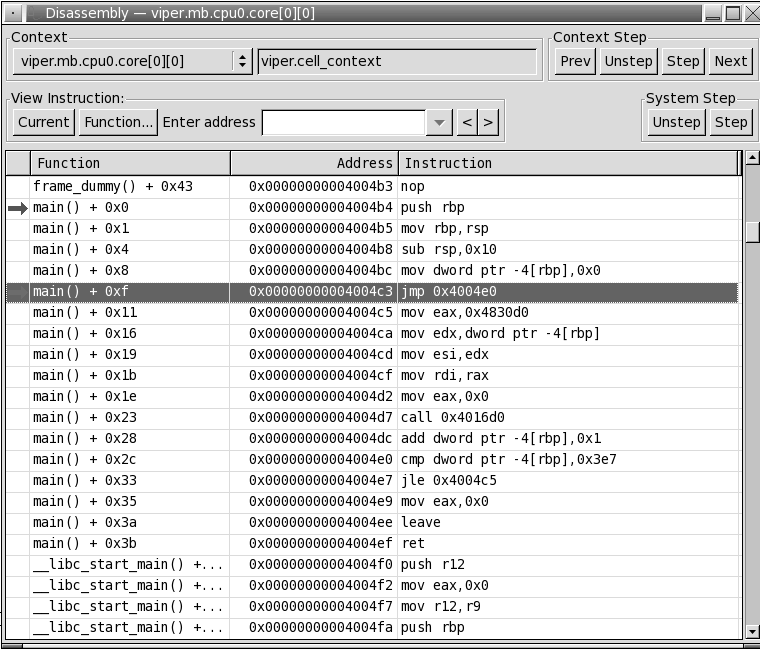
\includegraphics[width=0.6\textwidth]{./images/win-disassembly.png}
    \caption{Окно дизассемблера}
    \label{fig:win-disassembly}
\end{figure}

\begin{figure}[htb]
    \centering
    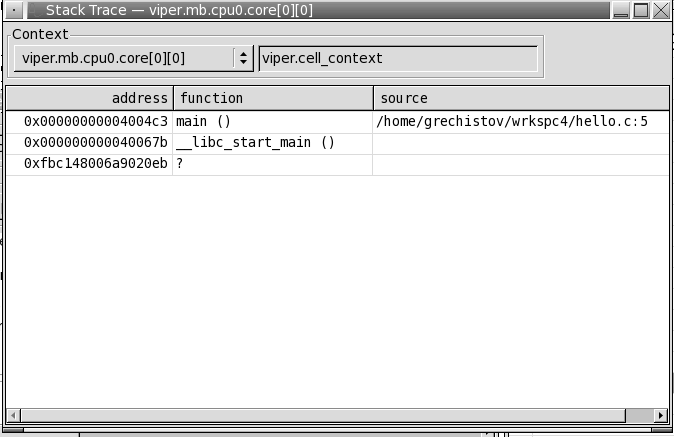
\includegraphics[width=0.6\textwidth]{./images/win-stack-trace.png}
    % win-stack-trace.png: 674x437 pixel, 96dpi, 17.83x11.56 cm, bb=0 0 505 328
    \caption{Окно просмотра стека}
    \label{fig:win-stack-trace}
\end{figure}


\subsection{Управление исполнением программы}

Теперь, когда симуляция находится внутри интересующей нас программы, отладчик должен позволять инспектировать состояние её переменных, положение указателя текущей инструкции, а также управлять пошаговым исполнением её операций. Для нас окажутся полезными следующие команды Simics.

\begin{enumerate*}
    \item \texttt{sym} --- получить значение переменной, определённой в текущем контексте гостевой программы.
\begin{lstlisting}
simics> sym argc
1
\end{lstlisting}

\item \texttt{step-line} --- выполнить одну строку исходного кода отлаживаемой программы и остановиться.
\item \texttt{next-line} --- выполнить одну строку исходного кода отлаживаемой программы и остановиться, при этом пропустив выполнение подпроцедур, если они вызываются.
\item \texttt{pos} --- узнать адрес функции или строки кода:
\begin{lstlisting}
simics> pos main
0x804832e
simics> pos debug_example.c:5
0x8048260
\end{lstlisting}

\end{enumerate*}

Кроме задания этих команд, управление исполнением может осуществляться с помощью кнопок \textbf{Step} и \textbf{Next} окна Disassembly (рис.~\ref{fig:win-disassembly}).

\subsubsection{Использование точек останова}

\paragraph{Доступы в память.}

Самый простой и часто используемый тип --- это точка останова по виртуальному адресу исполняемой инструкции:

\begin{lstlisting}
simics> break 0x4004b4
Breakpoint 1 set on address 0x4004b4 in 'viper.cell_context' with access mode 'x'
\end{lstlisting}

Кроме инструкций, точки останова могут быть созданы для регионов данных, при этом попытка гостевой программы обратиться к такому региону вызовет остановку симуляции. Формат команды при этом включает дополнительные флаги \texttt{-r} и \texttt{-w} для указания, должна ли она реагировать на чтение или запись памяти:

\begin{lstlisting}
simics> break 0x7fffdc2b3d7c -r -w
Breakpoint 2 set on address 0x7fffdc2b3d7c  in 'viper.cell_context' with access mode 'rw'
\end{lstlisting}

Полный формат команды \texttt{break} позволяет выбрать любую комбинацию флагов, а также указать длину наблюдаемого диапазона в байтах:
\begin{lstlisting}
break <address> [length] [-r] [-w] [-x]
\end{lstlisting}

Для того чтобы увидеть данные обо всех установленных точках останова, используется команда \texttt{list-breakpoints}.

\paragraph{Исключения.}

Другой класс событий, который может наблюдаться в отладчике, --- это архитектурные исключения. Для установки таких точек используется команда:

\begin{lstlisting}
break-exception name = Page_Fault_Exception
\end{lstlisting}

Полный список допустимых событий достаточно длинен; нас будут интересовать следующие из них: \texttt{Page_Fault_Exception}, \texttt{General_Protection_Exception}, \texttt{Invalid_Opcode_Exception}.

Точка останова прерывает исполнение симуляции. Если вместо этого желательно просто наблюдать за происходящими событиями, то следует использовать команду \texttt{trace-exception}, синтаксис который аналогичен \texttt{break-exception}.

\section{Задания}

\begin{enumerate*}

    \item Начать симуляцию и передать исследуемую программу в гостевую систему.
    \item Охарактеризовать тип проблемы, возникающий при работе программы.
    \item Отладить программу с помощью Simics.
\end{enumerate*}

\section{Вопросы для самостоятельного изучения}

\begin{enumerate*}
\item Для того чтобы любой отладчик, в том числе вcтроенный в Simics, мог иметь информацию об исходном коде исследуемой программы, информация о нём должна быть доступна ему на этапе отладки. В свою очередь программа должна быть скомпилирована с  использованием особенных флагов компиляции. Выясните, какие опции должны быть использованы в случае использования компилятора GCC.

\item Для того чтобы программа, скомпилированная на хозяйской системе, могла быть успешно запущена внутри гостя, требуется соблюсти несколько условий. Одно из них --- использование т.н. статической линковки, в случае GCC обозначаемой флагом \mbox{\texttt{-static}}. Выясните, зачем был использован этот флаг. При каких условиях на гостевую и хозяйскую системы можно использовать динамическую линковку?

\end{enumerate*}

\iftoggle{webpaper}{
    \printbibliography[title={Список литературы к занятию}]
}{}

\chapter{Моделирование платформы с архитектурой CHIP16}\label{chap:lab05}

Данная индивидуальная работа посвящена реализации модели компьютерной платформы, основанной на спецификации CHIP16~\cite{chip16-ngemu} --- полностью виртуальной системы, предназначенной для запуска простых видеоигр. Модель строится на основе API Simics и оформляется как набор модулей и сценариев для данного симулятора.

\section{Исходные спецификации CHIP16}

CHIP16 --- это RISC-подобный процессор фон-Неймана, работающий на частоте 1~МГц, имеющий 64 кбайт ОЗУ, со спрайтовой 16-цветной графикой разрешением 320×240, джойстиками с 8 кнопками и одноканальной звуковой картой.

\subsection{Существующие приложения}

\begin{itemize}
    \item Референсный симулятор --- \textsc{mash16}~\cite{chip16-mach16}.
    \item Описание устройств, набора инструкций и периферии~\cite{chip16-machspec}.
    \item Готовые образы памяти с приложениями, собранными для этой архитектуры~\cite{chip16-roms}.
\end{itemize}

\section{Структурная схема платформы}

Базовые узлы системы показаны на рис.~\ref{fig:chip16-platform}. Каждый обозначенный блок представляет собой один класс Simics, имя которого стоит после двоеточия.

\begin{figure}[htbp]
\centering
\begin{tikzpicture}[>=latex, node distance=0.5cm, font=\small]
\begin{scope}[minimum width=4cm]
    \node[draw] (cpu) {\textsc{cpu}: chip16};
    \node[draw, below = of cpu.south west, anchor=north west] (graph) {\textsc{graphics}: graph16};
    \node[draw, below = of graph.south west, anchor=north west] (sound) {\textsc{sound}: snd16};
    \node[draw, below = of sound.south west, anchor=north west] (joystick) {\textsc{joystick}: input16};
\end{scope}
    
\begin{scope}[minimum width = 3.9cm, inner xsep = 0pt]
     \node[draw, rotate=90, right = 1cm of joystick.south east, anchor=north west] (memory-space) {\textsc{cspace}: memory-space};
    \node[draw, rotate=90, right = 1cm of memory-space.south, anchor = north] (ram) {\textsc{ram}: ram};
    
    \node[draw, rotate=90, left = 1cm of cpu.north west, anchor=south east] (video-space) {\textsc{vspace}: memory-space};
    \node[draw, rotate=90, left = 1cm of video-space.south, anchor = south] (video-ram) {\textsc{video-ram}: ram};
\end{scope}

\draw[<->] (cpu.east) -- (cpu.east -| memory-space.north);
\draw[<-] (graph.east) -- (graph.east -| memory-space.north);
\draw[<-] (sound.east) -- (sound.east -| memory-space.north);
\draw[->] (joystick.east) -- (joystick.east -| memory-space.north);
\draw[<->] (graph.west) -- (graph.west -| video-space.south);

\draw[<->] (memory-space) -- (ram);
\draw[<->] (video-space) -- (video-ram);

\draw[->] (graph) -- (cpu) node[midway, right] {\tiny\texttt{VBLANK}};

\end{tikzpicture}
\caption{Схема соединения блоков}\label{fig:chip16-platform}
\end{figure}

\section{Модификации спецификации для полноплатформенной модели}

Оригинальная документация не описывает некоторые важные для практического построения детали взаимодействия узлов. Поэтому для нужд задания вводятся уточнения по принципам работы ряда узлов.

\paragraph{VBLANK.} Инструкция \textsc{vblank} введена для синхронизации ЦПУ с видеопроцессором. В данной работе её семантика изменена. \textsc{vblank} вызывает остановку процессора до поступления следующего прерывания.

\paragraph{Прерывания.} Для обеспечения работы \textsc{vblank} используется прерывание от видеокарты до процессора.

\paragraph{Инструкции DRW, PAL, SNG, CLS, BGC, SPR, FLIP, SNDx, SNP}. Данные инструкции предназначены для работы с периферией (видео и звуком). Для их реализации необходимо иметь однонаправленный канал для передачи сообщений. Для этих нужд используется  часть резервированного диапазона адресов I/O. Карта памяти выглядит следующим образом.

\todo Описать форматы пакетов аудио- и видеосообщений.

\begin{tabular}{rrl}
Диапазон адресов         & Длина & Назначение \\
\texttt{0x0000 -- 0xfdef}& 65008 & ОЗУ        \\
\texttt{0xfdf0 -- 0xffef}& 512   & Стек       \\
\texttt{0xfff0 -- 0xfff1}& 2     & Джойстик 1 \\
\texttt{0xfff2 -- 0xfff3}& 2     & Джойстик 2 \\
\texttt{0xfff4 -- 0xfff5}& 2     & Звуковая карта \\
\texttt{0xfff6 -- 0xfff9}& 4     & Видеокарта \\
\texttt{0xfffa -- 0xffff}& 6     & Зарезервировано \\
\end{tabular}


\section{Ход работы}

В данной секции разобраны общие вопросы организации разработки.
\subsection{Технология разработки}

\begin{itemize}
\item Хранение кода --- в SVN \todo{URL}. Лицензия кода --- закрытая, согласно договору предоставления Intel Academic SLA 1.0 (см. пункт 6.2). 

\item Документация --- в вики \todo{URL}. Лицензия документации --- CC BY-SA.

\item Распределение задач --- по одному модулю Simics на одного--двух выполняющих.
\item Промежуточная проверка качества --- юнит тесты для отдельных устройств.
\item Финальный продукт работы --- набор моделей и связывающий их скрипт (построенный на основе стандартной цели cosim)
\end{itemize}

\subsection{ЦПУ}

Основа для модели --- модифицированный \texttt{sample-risc}. \todo Подготовить код.

\subsection{Видеоконтроллер}

Основа для модели --- \texttt{sample-device-c}. Отрисовка изображения производится через SDL. Пример работы с экраном и клавиатурой из SDL: \url{http://www.aaroncox.net/tutorials/2dtutorials/sdlkeyboard.html}. Для 2.0: \url{http://www.sdltutorials.com/sdl-tutorial-basics}, \url{https://wiki.libsdl.org/MigrationGuide}.

\subsection{Джойстик}

Основа для модели --- \texttt{sample-device-c}. Ввод с хозяйской клавиатуры производится через SDL.

\section{Минимум и максимум цели проекта}

В зависимости от полноты выполнения студентами подзадач проекта выделяются следующие вехи, обозначающие достижение следующей ступени к симуляции, по сравнению с референсной моделью \textsc{mash16}.

\begin{enumerate}
    \item Модель способна исполнять образ памяти, написанный участниками проекта.
    \item Модель способна исполнять образ памяти из директории Demo (графическое приложение без звука и ввода).
    \item Модель способна исполнять образ памяти из директории Demo (графическое приложение со звуком и без ввода).
    \item Модель способна исполнять образ памяти из директории Games (графическое приложение со звуком и вводом с джойстика).
\end{enumerate}

% \subsection{Предложения для расширения архитектуры CHIP16}
% 
% \paragraph{Таймер.} Программируемый таймер.
% 
% \paragraph{Клавиатурный ввод.}
% 
% \paragraph{Дисковый накопитель.}
% 
% \paragraph{Контроллер прерываний.}


\section{init скрипт для старта и остановки демона лицензий}
Данный скрипт \texttt{lmgrd-simics} должен быть размещён в /etc/inid.d с правом исполнения, затем для Debian-систем должен быть включён с помощью команды:

\texttt{\# update-rc.d lmgrd-simics defaults}

Он доступен по ссылке \url{https://gist.github.com/grigory-rechistov/11142235}.

\begin{lstlisting}
#! /bin/sh
### BEGIN INIT INFO
# Provides:          lmgrd-simics
# Required-Start:    $remote_fs $syslog
# Required-Stop:     $remote_fs $syslog
# Default-Start:     2 3 4 5
# Default-Stop:      0 1 6
# Short-Description: Control Flexera lmgrd license daemon for Simics installation
# Description:       Control start/stop of lmgrd entry for Simics
#
### END INIT INFO

# Author: Grigory Rechistov (<grigory.rechistov@phystech.edu>)
#

# Do NOT "set -e"

# PATH should only include /usr/* if it runs after the mountnfs.sh script
PATH=/sbin:/usr/sbin:/bin:/usr/bin
DESC="lmgrd for Simics"
SIMICSDIR=/opt/simics/simics-4.6/simics-4.6.100
LICENSEFILE=/opt/simics/simics-4.6/simics-4.6.100/licenses/simics.lic # change to your license file
NAME=lmgrd
VENDORDAEMON=simics
DAEMONDIR=$SIMICSDIR/flexnet/linux64/bin
SCRIPTNAME=/etc/init.d/$NAME
DAEMON=$DAEMONDIR/$NAME

PIDFILE=/var/tmp/$NAME.pid
LOCKFILE=/var/tmp/locksimics
LOGFILE=/var/tmp/lmgrd-simics.log

# Exit if the package is not installed
[ -x "$DAEMON" ] || exit 0

# Read configuration variable file if it is present
[ -r /etc/default/$NAME ] && . /etc/default/$NAME

# Load the VERBOSE setting and other rcS variables
. /lib/init/vars.sh

# Define LSB log_* functions.
# Depend on lsb-base (>= 3.2-14) to ensure that this file is present
# and status_of_proc is working.
. /lib/lsb/init-functions

#
# Function that starts the daemon/service
#
do_start()
{
  # Return
  #   0 if daemon has been started
  #   1 if daemon was already running
  #   2 if daemon could not be started
  start-stop-daemon --start -c daemon:daemon --make-pidfile --pidfile $PIDFILE -d $DAEMONDIR --exec $DAEMON -- -c $LICENSEFILE -l +$LOGFILE || return 2
  pidof $NAME > $PIDFILE # This is lame; but lmgrd about itself does not create anything.
}

#
# Function that stops the daemon/service
#
do_stop()
{
  # Return
  #   0 if daemon has been stopped
  #   1 if daemon was already stopped
  #   2 if daemon could not be stopped
  #   other if a failure occurred
  start-stop-daemon --stop --retry=TERM/30/KILL/5 --pidfile $PIDFILE --name $NAME
  RETVAL="$?"
  [ "$RETVAL" = 2 ] && return 2
  # Many daemons don't delete their pidfiles when they exit.
  rm -f $PIDFILE
        rm -f $LOCKFILE
  return "$RETVAL"
}

#
# Function that sends a SIGHUP to the daemon/service
#
do_reload() {
  #
  # If the daemon can reload its configuration without
  # restarting (for example, when it is sent a SIGHUP),
  # then implement that here.
  #
  start-stop-daemon --stop --signal 1 --quiet --pidfile $PIDFILE --name $NAME
  return 0
}

case "$1" in
  start)
  [ "$VERBOSE" != no ] && log_daemon_msg "Starting $DESC" "$NAME"
  do_start
  case "$?" in
    0|1) [ "$VERBOSE" != no ] && log_end_msg 0 ;;
    2) [ "$VERBOSE" != no ] && log_end_msg 1 ;;
  esac
  ;;
  stop)
  [ "$VERBOSE" != no ] && log_daemon_msg "Stopping $DESC" "$NAME"
  do_stop
  case "$?" in
    0|1) [ "$VERBOSE" != no ] && log_end_msg 0 ;;
    2) [ "$VERBOSE" != no ] && log_end_msg 1 ;;
  esac
  ;;
  status)
       status_of_proc "$DAEMON" "$NAME" && exit 0 || exit $?
       ;;
  #reload|force-reload)
  #
  # If do_reload() is not implemented then leave this commented out
  # and leave 'force-reload' as an alias for 'restart'.
  #
  #log_daemon_msg "Reloading $DESC" "$NAME"
  #do_reload
  #log_end_msg $?
  #;;
  restart|force-reload)
  #
  # If the "reload" option is implemented then remove the
  # 'force-reload' alias
  #
  log_daemon_msg "Restarting $DESC" "$NAME"
  do_stop
  case "$?" in
    0|1)
    do_start
    case "$?" in
      0) log_end_msg 0 ;;
      1) log_end_msg 1 ;; # Old process is still running
      *) log_end_msg 1 ;; # Failed to start
    esac
    ;;
    *)
      # Failed to stop
    log_end_msg 1
    ;;
  esac
  ;;
  *)
  #echo "Usage: $SCRIPTNAME {start|stop|restart|reload|force-reload}" >&2
  echo "Usage: $SCRIPTNAME {start|stop|status|restart|force-reload}" >&2
  exit 3
  ;;
esac
:
\end{lstlisting}


\iftoggle{webpaper}{
    \printbibliography[title={Список литературы к занятию}]
}{}

\appendix
\appendixpage

\chapter{Дополнительная информация по работе с~Simics} \label{chap:append01}

В данное приложение включены сведения о различных приёмах, используемых при ежедневном использовании Simics, не описанные в главах, посвящённых индивидуальным лабораторным работам. Данный материал не заменяет необходимость ознакомления с официальной документацией Simics, а лишь подчёркивает ключевые моменты в ней.

\section{Обновление workspace}

Для получения последних исправлений ошибок в моделях необходимо использовать самую свежую версию базового пакета Simics из  установленных на системе. Номера доступных версий можно определить по именам существующих директорий (по умолчанию в \texttt{/opt/simics}). В дальнейших примерах последней версией будет считаться \textbf{4.6.32}, при этом 4.6 --- это основная версия, а последняя цифра --- номер минорной версии обновления, котороый будет использован ниже.

Каждая копия workspace характеризуется \emph{комбинацией} версий пакетов, в ней используемых. Версия пакета Simics Base (\textnumero 1000) определяет настройки версий остальных пакетов, установленных одновременно с ним. Для того, чтобы увидеть список установленных пакетов и их версии, используйте ключ \texttt{-v} при запуске Simics:

\begin{lstlisting}
$ ./simics -v
Simics Base                                        1000    4.6.32    (4051)
Model Library: Intel Core i7 with X58 and ICH10    2075    4.6.21    (4051)
Model Builder                                      1010    4.6.14    (4051)
Extension Builder                                  1012    4.6.6     (4042)
\end{lstlisting}

Также версию Simics можно узнать из командной строки любой уже запущенной симуляции c помощью команды \texttt{version}:

\begin{lstlisting}
simics> version
Installed Products:

Model Builder
Extension Builder
Model Library: Intel Core i7 with X58 and ICH10

Installed Packages:

Package                  Nbr  Version  Build  Sources
=====================================================
Simics-Base             1000  4.6.32    4145       No
Model-Builder           1010  4.6.49    4146       No
Extension-Builder       1012  4.6.19    4141       No
x86-Core-i7-X58-ICH10   2075  4.6.59    4146       No
\end{lstlisting}

В примере сверху базовый пакет имеет версию 4.6.32. Обновления пакетов могут периодически устанавливаться в вашей системе для исправления ошибок в предоставляемых моделей. Однако уже созданные workspace будут по-прежнему использовать старые версии, если для них не выполнить процедуру обновления. 

Для обновления workspace, как и для его создания, используется программа \texttt{workspace-setup}, находящаяся внутри новой версии базового пакета (версии 4.6.\textbf{<minor>}).

\begin{lstlisting}
$ /opt/simics/simics-4.6/simics-4.6.<minor>/bin/workspace-setup
Workspace updated successfully
\end{lstlisting}

\section{Список часто используемых команд Simics}

\begin{center}
\small
\begin{tabularx}{\textwidth}{Xlp{0.4\textwidth}}
%\begin{longtable}{|p{0.3\textwidth}|l|p{0.3\textwidth}|}\
\textbf{Команда}                          & \textbf{Синонимы}  & \textbf{Выполняемая функция}\\\hline
\texttt{help <topic>}                     & \texttt{man}       & Справка по команде, классу или слову topic\\
\texttt{win-help}                         &                    & Открыть окно индексируемой справки \\
\texttt{continue}                         & \texttt{c, r, run} & Начать или продолжить симуляцию\\
\texttt{stop}                             &                    & Остановить симуляцию\\
\texttt{step-cycle [count]}               & \texttt{sc}        & Исполнить count циклов, печатаю следующую инструкцию\\
\texttt{exit}                             & \texttt{quit, q}   & Выйти из симулятора\\
\texttt{run-command-file <script.simics>} &                    & Выполнить скрипт Simics\\
\texttt{pregs [-all]}                     &                    & Распечатать содержимое регистров текущего процессора\\
\texttt{print-time [-all]}                & \texttt{ptime}     & Вывести значение виртуального времени процессора\\
\texttt{win-control}                      &                    & Открыть окно \textbf{Simics Control}\\
\texttt{\%<register name>}                & \texttt{read-reg}  & Прочитать содержимое регистра текущего процессора \\
\texttt{\%<register name> = <val>}        & \texttt{write-reg} & Записать значение в регистр текущего процессора \\
\texttt{output-radix <10|16>}             &                    & Изменить основание используемой для вывода чисел системы счисления\\
\texttt{break <address>}                  &                    & Поставить точку останова по адресу \\
\texttt{delete [id]}                      &                    & Удалить точку останова по её номеру \\
\end{tabularx}

% \end{longtable}
\end{center}



\chapter{Скрипт для отладки}\label{chap:app-broken-script}

\begin{lstlisting}
name_prefix = cli.simenv.host_name
if name_prefix != "":
    name_prefix = name_prefix + "_"

sample_risc0 = pre_conf_object(name_prefix + "sample_risc0", "sample-risc")
sample_risc0.queue = sample_risc0

ram_image0 = pre_conf_object(name_prefix + "ram_image0", "image")
ram_image0.queue = sample_risc0
ram_image0.size = 0x800000

ram0 = pre_conf_object(name_prefix + "ram0", "ram")
ram0.image = ram_image0

phys_mem0 = pre_conf_object(name_prefix + "phys_mem0", "memory-space")
phys_mem0.queue = sample_risc0
phys_mem0.map = [[     0x0, ram0,                 0, 0, 0x800000],
                ]

ctx0 = pre_conf_object(name_prefix + "ctx0", "context")
ctx0.queue = sample_risc0

sample_core0 = pre_conf_object(name_prefix + "sample_core0", "sample-risc-core")
sample_core0.queue = sample_risc0
sample_core0.sample_risc = sample_risc0
sample_core0.physical_memory_space = phys_mem0
sample_core0.current_context = ctx0

#cosim_cell = pre_conf_object(name_prefix + "cosim_cell", "cell")
#cosim_cell.current_processor = sample_core0
#cosim_cell.current_step_obj = sample_risc0
#cosim_cell.current_cycle_obj = sample_risc0
#cosim_cell.scheduled_object = sample_risc0
#sample_risc0.cell = cosim_cell

SIM_add_configuration([sample_risc0, ctx0, ram_image0, ram0, phys_mem0, sample_core0, sample_core1], None)
\end{lstlisting}

\chapter{Код целевого скрипта practicum.simics}\label{chap:target-script}

\begin{lstlisting}
# Script for mipt practicum
load-module pci-components
load-module std-components
load-module x86-comp
load-module x86-nehalem-comp
load-module x58-ich10-comp
load-module memory-comp

add-directory "%simics%/targets/x86-x58-ich10/images/"

$disk_image         = "/share_debian/hpc-images/debian-master-2012-05-12.craff"
$cpu_class          = core-i7-single
$freq_mhz           = 3300
$cpi                = 1
$disk_size          = 20496236544
$rtc_time           = "2008-06-05 23:52:01 UTC"
$memory_megs        = 2048
$text_console       = TURE
$use_acpi           = TRUE
$gpu                = "accel-vga"
$bios               = "seabios-simics-x58-ich10-0.6.0-20110324.bin"
$break_on_reboot    = TRUE
$apic_freq_mhz      = 133
$use_vmp            = TRUE
$spi_flash          = "spi-flash.bin"
$mac_address        = "00:19:A0:E1:1C:9F"
$host_name          = "practicum"

$system = (create-x86-chassis name = $host_name)

### motherboard
$motherboard = (create-motherboard-x58-ich10 $system.mb
        rtc_time = $rtc_time
        acpi = $use_acpi
        break_on_reboot = $break_on_reboot
        bios = $bios
	    mac_address = $mac_address
        spi_flash = $spi_flash)
$southbridge = $motherboard.sb
$northbridge = $motherboard.nb

### processor
$create_processor = "create-processor-" + $cpu_class
$create_processor_command = (
        $create_processor
        + " $motherboard.cpu0"
        + " freq_mhz = $freq_mhz"
        + " apic_freq_mhz = $apic_freq_mhz"
        + " use_vmp = $use_vmp"
        + " cpi = $cpi")
$cpu0 = (exec $create_processor_command)
connect $motherboard.socket[0] $cpu0.socket

### memory
$dimm = (create-simple-memory-module $motherboard.memory
                                      memory_megs = $memory_megs)
connect $motherboard.dimm[0] $dimm.mem_bus

### GPU
$vga = (create-pci-accel-vga $motherboard.gpu)
connect $northbridge.gpu $vga.connector_pci_bus

### consoles
$console = (create-std-text-graphics-console $system.console)
$console.connect keyboard $southbridge
$console.connect $vga

### disk
if not (lookup-file $disk_image) {
    interrupt-script "Disk image file not found: " + $disk_image
}
$disk = (create-std-ide-disk $system.disk size = $disk_size file = $disk_image)
$southbridge.connect "ide_slot[0]" $disk

instantiate-components

#SimicsFS support (add SimicsFS pseudo device)
$hostfs = python "SIM_create_object('hostfs', 'hfs0', [])"
practicum.mb.phys_mem.add-map $hostfs 0xfed2_0000 16

try {
    win-command-line
} except { echo "Failed to create GUI"}

script-branch { # Automatize GRUB and login
    local $con = $host_name.console.con
    $con.wait-for-string "automatically in 5s"
    $con.input "\n"
    $con.wait-for-string "login:"
    $con.input "user\n"
    $con.wait-for-string "Password:"
    $con.input "user\n"
}

\end{lstlisting}

\chapter{Программа debug_example.c}\label{chap:debug-example}

\begin{lstlisting}
/*
 * This program  reads input and converts it to uppercase.
 * It has an intentional bug included that makes it crash on certain inputs.
 * 
 * Usage: stdin - input string.
 * Compile with gcc -static -g debug_example.c -o debug_example
 */
	
#include <stdio.h>
#include <string.h>
#include <stdlib.h>

void read_input(char* in) {
    char symbol;
    in[0] = 0; // initialize the string with zero length
    while((symbol = getchar()) != EOF) {
        *in++ = symbol;
    }
    *in = 0; // close the string
}

void convert_to_uppercase(char * in, char *out) {
    int i;
    for (i =0; i <= strlen(in); i++) {
        if (isalpha(in[i]))
            out[i] = toupper(in[i]);
        else
            out[i] = in[i];
    }
}

int main(int argc, char** argv) {
    char input[32], *output;
    
    read_input(input);
    convert_to_uppercase(input, output);
    
    printf("%s\n", output);
    return 0;
}
\end{lstlisting}


\chapter{Установка и лицензирование Simics} \label{chap:installation-notes}

В данное приложение включена информация по лицензированию и установке Simics в учебной лаборатории. Наиболее полная информация по данному вопросу содержится в документе «Simics Installation Guide», который идёт в поставке с пакетами Simics (файл  \texttt{installation-guide.pdf}).

Приводимые ниже инструкции были собраны для Simics версии 4.6 для хозяйской системы Linux 64 бит, рекомендуемой для всех пользователей. Для ОС Linux 32 бит инструкции изменяются незначительно; для ОС Windows они применимы после учёта особенностей графического процесса инсталляции.

\section{Академическая программа Wind River Simics}

\todo

\section{Получение и продление лицензии}

\todo

\subsection{Условия предоставления}

Использование Simics по академической программе должно строго соответствовать условиям соглашения, т.е. быть ограничено учебной и/или некоммерческой научно-исследовательской деятельностью. В случае возникновения необходимости проведения коммерческих исследований или разработок необходимо обратиться к представителям Wind River для получения нового соглашения и типа лицензии.

Держатель лицензии от участвующего университета обязан донести эту информацию до всех пользователей инсталляции и контролировать выполнение ими условий соглашения, в том числе с помощью административных и технических мер.

\todo ограничения файервола
\todo Порты

\section{Установка файлов и запрос лицензии}

\subsection{Пакеты}

Simics распространяется в формате пакетов --- набора файлов, реализующих одну или несколько типов моделируемых систем или функциональность самого симулятора. Каждый пакет имеет свой фиксированный номер. Пакет \textnumero 1000 --- это Simics Base, содержащий базовую функциональность симулятора. Все остальные пакеты являются дополнениями к нему.

Дистрибутив пакета --- это файл с именем вида \texttt{simics-pkg-1000-4.6.34-linux64.tar}.  Здесь 1000 --- номер пакета, 4.6.34 --- версия пакета, linux64 --- архитектура хозяйской системы. Каждый дистрибутив каждого пакета зашифрован собственным ключом, состоящим из 32 символов. Дистрибутивы и их ключи получите у спонсора вашей академической программы.

Для установки всех необходимых файлов выполняется следующая процедура. Часть команд может потребовать наличия прав администратора.

\begin{enumerate}
\item Разархивируйте все пакеты *.tar:
\begin{lstlisting}
$for f in simics-pkg-*.tar; do tar xf $f; done
\end{lstlisting}
\item В созданной директории \texttt{simics-4.6-install} запустите скрипт установки:
\begin{lstlisting}
$ cd simics-4.6-install
# ./install-simics.pl
\end{lstlisting} 
    
\item Введите ключи шифрования для каждого номера пакета, который планируется установить:
\begin{lstlisting}
-> Looking for Simics packages in current directory...
Enter a decryption key for package-1000-4.6.34-linux64.tar.gz.tf,
or Enter to [Abort]: [Ключ]
\end{lstlisting} 

\item На вопрос, какие из пакетов требуется установить, ответьте <<All packages>>:
\begin{lstlisting}
install-simics can install the following packages:
 Number  Name          Type    Version  Host     Package
   1     Simics-Base   simics  4.6.34   linux64  package-1000
   2     Eclipse       addon   4.6.16   linux64  package-1001
   3     All packages
Please enter the numbers of the packages you want to install, as in "1 4 3"
Package numbers, or Enter to [Abort]:  3
\end{lstlisting}
    
\item На вопрос о директории назначения введите абсолютный путь или оставьте значение по умолчанию:
\begin{lstlisting}
Enter a destination directory for installation, or Enter
for [/opt/simics]:  [Путь установки или Enter]
\end{lstlisting}

\item Подтвердите начало установки, выбрав <<y>>.

\item При введении правильных ключей дистрибутивы будут расшифрованы и установлены в указанную при установке директорию --- в ней должны появиться подпапки с файлами из пакетов Simics.
\begin{lstlisting}
-> Decrypting package-1000-4.6.34-linux64.tar.gz.tf
-> Testing package-1000-4.6.34-linux64.tar.gz
-> Installing package-1000-4.6.34-linux64.tar.gz
-> Decrypting package-1001-4.6.16-linux64.tar.gz.tf
-> Testing package-1001-4.6.16-linux64.tar.gz
-> Installing package-1001-4.6.16-linux64.tar.gz

===============================

install-simics has finished installing the packages and will now
configure them.

No previous Simics installation was found. If you wish to configure
the newly installed Simics from a previous installation not found by
this script, you can do so by running the 'addon-manager' script in
the Simics installation with the option --upgrade-from:
    ./bin/addon-manager --upgrade-from /previous/install/

install-simics has installed the following add-on package:
   Eclipse  4.6.16  /opt/simics/simics-eclipse-4.8.26
\end{lstlisting}

\item На вопрос о регистрации расширений (\abbr add-on) ответьте <<y>>:
\begin{lstlisting}
Do you wish to make these add-on packages available in
Simics-Base 4.6.34? (y, n) [y]:  y
\end{lstlisting}   
\end{enumerate}

После успешного завершения файлы Simics были скопированы на ваш диск. Следующий шаг --- получение лицензии для их запуска. Он описывается далее.

\subsection{Получение lmhostid}

Для получения файла лицензии необходимо сгенерировать и передать число, так называемый lmhostid

\paragraph{Об именовании сетевых интерфейсов.} На момент написания данного материала утилиты из состава Simics не поддерживали получение корректного lmhostid на системах, использующих схему «стабильного именования» сетевых интерфейсов. Вместо традиционных для Linux имён \texttt{eth0}, \texttt{eth1} и т.д. сетевым картам выдаются имена, зависящие от производителя и физического расположения в системе.

Для обеспечения \todo

\begin{enumerate}
    \item Установите пакет \texttt{lsb-core} на системе. Для Debian и Ubuntu это выполняется командой 
    
    \texttt{\# apt-get install lsb-core}
         
    \item Для получения lmhostid на сервере, \textit{который будет использоваться для запуска демона лицензий}, выполните команду:
    
\begin{lstlisting}
$ /opt/simics/simics-4.6.34/flexnet/linux64/bin/lmutil lmhostid
lmutil - Copyright (c) 1989-2011 Flexera Software, Inc. All Rights Reserved.
The FlexNet host ID of this machine is ""602fe934a369 422fe934a36c ""
Only use ONE from the list of hostids.
\end{lstlisting}

Выданное число (в примере выше <<602fe934a369>>) --- это lmhostid. Если чисел выдано несколько, то используйте только одно из них.
    
\end{enumerate}


Возможные решения:



\todo{Команда}

\subsection{Заполнение заявки}




\section{Настройка сервера лицензий}


\subsection{Файл лицензии}

Получаемый от производителя файл лицензии --- это текстовый документ, содержащий информацию о сроке действия, ограничениях количества одновременно запускаемых копий и поддерживаемых расширениях приложения. Пример содержимого для начала этого файла:

\begin{lstlisting}
# Simics 4.6 licence for the Simics Academic Program
#
# University:        Moscow Institute of Physics and Technology
# Contact:           academic.contact@university.edu
# Sponsor:           sponsor.contact@sponsor.com
# Licensing Contact: licencing.contact@licencer.com
#
SERVER  lic.university.edu lmhostid
VENDOR simics /home/Incoming/simics-4.6/simics-4.6.100/flexnet/linux64/bin
#
FEATURE simics simics 4.6 28-feb-2014 50 BD47D265FA68 \
        VENDOR_STRING=intel;academic HOSTID=ANY BORROW TS_OK \
        SIGN="0441 6AFA 450C BDBE E4D7 E125 1042 EEFF 04B5 767A ABCD \
        5088 80DB D912 292E 4FD5 22DD 22D0 D55F 5B25 4818"
<...>
\end{lstlisting}

Не изменяйте никаких строчек этого файла, кроме имени сервера лицензий. Сохраните копию файла в надёжном месте. Запишите дату окончания действия лицензии для последующей своевременной инициации процедуры обновления.

\subsection{Запуск сервера}

\subsection{Проверка работоспособности}



\section{Расположение файлов и сервера лицензий при подключении по сети}

По умолчанию все файлы Simics размещаются в директории \texttt{/opt/simics}. Если необходимо обеспечить запуск симулятора на нескольких компьютерах, подсоединённых по сети, рекомендуется разместить эти файлы установки в файловой системе, доступной по сети, например, по протоколам NFS или CIFS. Таким образом, клиентские машины смогут переиспользовать структуру инсталляции без необходимости её копирования на локальные диски, что упростит поддержку и обновления. Настройка сетевой файловой системы выходит за рамки данного руководства; необходимую информацию можно найти, например, в~\cite{nfs}.

\subsection{Финальный вид инсталляции}

На рис.~\ref{fig:install-overview} приведена рекомендуемая схема соединения систем и расположения служб для работы Simics на всех компьютерах учебного класса или лаборатории. В данном примере сервер для запуска демона лицензий отделён от сервера общих файлов; на практике они могут быть одной и той же системой.

\begin{figure}[htbp]
\centering
\begin{tikzpicture}[>=latex, font=\small]
    
    \node[draw] (lic-file) {simics-00AA-2014.lic};
    \node[draw, below = 0.25cm of lic-file] (lmgrd) {lmgrd демон};
    \node[above = 0.25cm of lic-file] (lic-host) {lic.university.edu};
    \node[draw, fit = (lic-file) (lmgrd) (lic-host)] (lic-server) {};    
    
    \node[draw, below = 2cm of lic-server] (installation) {/opt/simics/...};
    \node[draw, below = 0.25cm of installation] (nfs) {NFS демон};
    \node[above = 0.25cm of installation] (nfs-host) {nfs.university.edu};
    \node[draw, fit = (installation) (nfs) (nfs-host)] (nfs-server) {};
    
    \node[draw, right = 3cm of lic-file] (simics01) {Симуляция};
    \node[draw, below = 0.25cm of simics01] (lab01-client) {Клиент Simics};
    \node[above = 0.25cm of simics01] (lab01-host) {lab01.university.edu};
    \node[draw, fit = (simics01) (lab01-client) (lab01-host)] (lab01) {};

    \node[draw, below = 1.5cm of lab01] (simics02) {Симуляция};
    \node[draw, below = 0.25cm of simics02] (lab02-client) {Клиент Simics};
    \node[above = 0.25cm of simics02] (lab02-host) {lab02.university.edu};
    \node[draw, fit = (simics02) (lab02-client) (lab02-host)] (lab02) {};

    \node[draw, below = 1.5cm of lab02] (simics03) {Симуляция};
    \node[draw, below = 0.25cm of simics03] (lab03-client) {Клиент Simics};
    \node[above = 0.25cm of simics03] (lab03-host) {lab03.university.edu};
    \node[draw, fit = (simics03) (lab03-client) (lab03-host)] (lab03) {};
    
    \draw[->] (lmgrd.east) -- (lab01-client.west);
    \draw[->] (lmgrd.east) -- (lab02-client.west);
    \draw[->] (lmgrd.east) -- (lab03-client.west);
    
    \coordinate[right = 1cm of installation]  (midpoint);
    \draw[<-] (installation) -| (midpoint);
    \draw[->] (midpoint) |- (simics01);
    \draw[->] (midpoint) |- (simics02);
    \draw[->] (midpoint) |- (simics03);
    
\end{tikzpicture}
\caption{Расположение и функции узлов инсталляции Simics}\label{fig:install-overview}
\end{figure}


\subsection{Решение возникших проблем}

\begin{description}
    \item[Невозможно стартовать lmgrd]
    
    \item[Невозможно запустить Simics]
    
    \item[Нет подключения к демону лицензии с сервера]

    
    \item[Нет подключения к демону лицензии по сети] 
    
    \item[Демон лицензий не работает после перезагрузки сервера] 
    
    
    \item[Исчерпано число лицензий]
    
\end{description}

\section{Обновление пакетов инсталляции}

\todo

\iftoggle{webpaper}{
    \printbibliography[title={Литература}]
}{}



\iftoggle{webpaper}{
    \section*{Список TODO}

Даннаяя секция предназначена для напоминания авторам, какие задачи по улучшению содержимого книги необходимо выполнить. Всем остальным просьба не обращать внимания.


} {
    \clearpage

\printbibliography[title={Литература}]

% Uncomment once to generate bbl, then adjust it by hand and input
% \bibliographystyle{ugost2008s}
% \bibliography{phd,mine}

%\input{bibliography-precompiled.tex}


\addcontentsline{toc}{chapter}{Литература}
    \thispagestyle{empty}
\begingroup
\small
\parindent=0pt % no indentation

\begin{center}

\begin{normalsize}
\textsf{Учебное издание}
\end{normalsize}

\vfill

\begin{large}
\textsf{ЛАБОРАТОРНЫЙ ПРАКТИКУМ \\
        \medskip
        ПО ПРОГРАММНОМУ МОДЕЛИРОВАНИЮ}
\end{large}

\vfill

\begin{normalsize}
Учебно-методическое пособие
\end{normalsize}

\vfill

\begin{small}
Составители:

\textbf{Юлюгин Евгений Андреевич, Речистов Григорий Сергеевич, \\
        Щелкунов Николай Николаевич, Гаврилов Дмитрий Александрович}
\end{small}

\end{center}

\vfill

\begin{flushleft}

\footnotesize

Редактор \textit{И.А. Волкова}. Корректор \textit{О.П. Котова}.

Подписано в печать 15.09.2013. Формат $60 \times 84 {^1}/_{16}$. Усл. печ. л. 2,75. Уч.-изд. л. 2,0.

Тираж 250 экз. Заказ № 182.

\medskip

Федеральное государственное автономное образовательное \\
учреждение высшего профессионального образования \\
<<Московский физико-тех\-ни\-чес\-кий институт (государственный университет)>>

141700, Московская обл., г. Долгопрудный, Институтский пер., 9

Тел. (495) 408-5822. E-mail: \url{rio@mail.mipt.ru}

\line(1,0){200}

Отдел оперативной полиграфии <<Физтех-полиграф>>

141700, Московская обл., г. Долгопрудный, Институтский пер., 9

Тел. (495) 408-8430. E-mail: \url{polygraph@miptic.ru}

\end{flushleft}
\endgroup
\phantomsection\label{page:lastpage}
}

\end{document}
